% This work is licensed under the Creative Commons Attribution-ShareAlike 4.0 International License.
% To view a copy of this license, visit http://creativecommons.org/licenses/by-sa/4.0/.

\documentclass[a4paper,12pt]{scrbook}
\usepackage[T1]{fontenc} % Include italic fonts
\usepackage{fontspec} % Compile with \XeLaTeX
\usepackage{geometry} % Page margins
\usepackage{titling} % Title page container
\usepackage{wrapfig} % Picture container
\usepackage{graphicx} % Including graphics
\usepackage{natbib}
\usepackage[colorlinks, allcolors=blue,xetex]{hyperref}
\usepackage{hyperxmp} % Import license metadata
\usepackage[acronym,toc,shortcuts,nohypertypes=acronym]{glossaries} % Acronyms
\usepackage{tikz} % Charts
\usepackage{subcaption} % Grid of figures
\usepackage{tabulary} % Autostretch columns
\renewcommand{\familydefault}{\sfdefault}
\bibliographystyle{apalike}

\title{Evaluating the potential of Sentinel-2 and Landsat image time series for detecting selective logging in the Amazon}
\author{Dainius Masiliūnas}
\date{\today}
\hypersetup{
    pdflicenseurl={http://creativecommons.org/licenses/by-sa/4.0/},
    pdfcopyright={This work is licensed under the Creative Commons Attribution-ShareAlike 4.0 International License.},
    pdfauthor={\theauthor}, % These are supposed to be the default but don't seem to be
    pdftitle={\thetitle},
    pdflang={en-GB}
}

% Flowchart blocks
\usetikzlibrary{shadows,arrows,positioning,shapes}
\tikzstyle{block} = [rectangle, draw, fill=white, 
    text width=8em, text centered, rounded corners, minimum height=3em]
\tikzstyle{line} = [draw, -latex']
\tikzstyle{data} = [trapezium, trapezium left angle=70, trapezium right angle=110, text centered, draw,
    text width=7em, fill=gray!30, double copy shadow, minimum height=3em]
\tikzstyle{datasingle} = [trapezium, trapezium left angle=70, trapezium right angle=110, text centered, draw,
    text width=8em, fill=gray!30]
\tikzstyle{bigdata} = [trapezium, trapezium left angle=80, trapezium right angle=100, text centered, draw,
    text width=14em, fill=gray!30, double copy shadow, minimum height=3em]

% Define acronyms
\newcommand{\underletter}[1]{\textbf{#1}} % Quick toggle of underlines
\newacronym{NDVI}{NDVI}{\underletter{N}ormalised \underletter{D}ifference \underletter{V}egetation \underletter{I}ndex}
\newacronym{REDD+}{REDD+}{\underletter{R}educing \underletter{E}missions from \underletter{D}eforestation and forest \underletter{D}egradation}
\newacronym{LAI}{LAI}{\underletter{L}eaf \underletter{A}rea \underletter{I}ndex}
\newacronym{EVI}{EVI}{\underletter{E}nhaced \underletter{V}egetation \underletter{I}ndex}
\newacronym{OLI}{OLI}{\underletter{O}perational \underletter{L}and \underletter{I}mager}
\newacronym{NBR}{NBR}{\underletter{N}ormalised \underletter{B}urn \underletter{R}atio}
\newacronym{NBR2}{NBR2}{\underletter{N}ormalised \underletter{B}urn \underletter{R}atio \underletter{2}}
\newacronym{NDMI}{NDMI}{\underletter{N}ormalised \underletter{D}ifference \underletter{M}oisture \underletter{I}ndex}
\newacronym{SAVI}{SAVI}{\underletter{S}oil \underletter{A}djusted \underletter{V}egetation \underletter{I}ndex}
\newacronym{MSAVI}{MSAVI}{\underletter{M}odified \underletter{S}oil \underletter{A}djusted \underletter{V}egetation \underletter{I}ndex}
\newacronym{TM}{TM}{\underletter{T}hematic \underletter{M}apper}
\newacronym{ETM+}{ETM+}{\underletter{E}nhanced \underletter{T}hematic \underletter{M}apper \underletter{Plus}}
\newacronym{WUR}{WUR}{\underletter{W}ageningen \underletter{U}niversity \& \underletter{R}esearch}
\newacronym{GPS}{GPS}{\underletter{G}lobal \underletter{P}ositioning \underletter{S}ystem}
\newacronym{GNSS}{GNSS}{\underletter{G}lobal \underletter{N}avigation \underletter{S}atellite \underletter{S}ystem}
\newacronym{NIR}{NIR}{\underletter{N}ear \underletter{I}nfra\underletter{r}ed}
\newacronym{SWIR}{SWIR}{\underletter{S}hort\underletter{w}ave \underletter{I}nfra\underletter{r}ed}
\newacronym{RIL}{RIL}{\underletter{R}educed-\underletter{I}mpact \underletter{L}ogging}
\newacronym{USGS}{USGS}{\underletter{U}.\underletter{S}. \underletter{G}eological \underletter{S}urvey}
\newacronym{UTM}{UTM}{\underletter{U}niversal \underletter{T}ransverse \underletter{M}ercator}
\newacronym{ESA}{ESA}{\underletter{E}uropean \underletter{S}pace \underletter{A}gency}
\newacronym{MSI}{MSI}{\underletter{M}ulti-\underletter{s}pectral \underletter{I}mager}
\newacronym{ASTER}{ASTER}{\underletter{A}dvanced \underletter{S}paceborne \underletter{T}hermal \underletter{E}mission and Reflection \underletter{R}adiometer}
\newacronym{SLC}{SLC}{\underletter{S}can \underletter{L}ine \underletter{C}orrector}
\newacronym{LP DAAC}{LP DAAC}{\underletter{L}and \underletter{P}rocesses \underletter{D}istributed \underletter{A}ctive \underletter{A}rchive \underletter{C}enter}
\newacronym{ESPA}{ESPA}{Earth Resources Observation and Science (\underletter{E}ROS) Center \underletter{S}cience \underletter{P}rocessing \underletter{A}rchitecture}
\newacronym{RGB}{RGB}{\underletter{R}ed, \underletter{G}reen, \underletter{B}lue}
\newacronym{DBH}{DBH}{\underletter{D}iameter at \underletter{B}reast \underletter{H}eight}
\newacronym{DEM}{DEM}{\underletter{D}igital \underletter{E}levation \underletter{M}odel}
\newacronym{SRTM}{SRTM}{\underletter{S}huttle \underletter{R}adar \underletter{T}opography \underletter{M}ission}
\newacronym{NA}{NA}{\underletter{N}ot \underletter{A}vailable}
\newacronym{GiB}{GiB}{\underletter{G}ib\underletter{i}\underletter{b}ytes}
\newacronym{RAM}{RAM}{\underletter{R}andom \underletter{A}ccess \underletter{M}emory}
\makenoidxglossaries

\geometry{top=1.25cm,bottom=0.96cm,inner=2cm,outer=1.91cm,foot=0cm,includeheadfoot} % First page margins
\begin{document}
 \begin{titlingpage}
  {\Large Geo-information Science and Remote Sensing}\vspace{0.9cm}
  
  {\Large Thesis Report GIRS-2017-xx}\vspace{0.9cm}
  
  \hrule\vspace{1.1cm}
  
  {\bfseries \Large \MakeUppercase{\thetitle}}\vspace{2.0cm}
  
  \begin{wrapfigure}{r}{0.55\textwidth}
    \vspace{1cm}
    \includegraphics[height=9.5cm,draft]{title/picture.png}
  \end{wrapfigure}
  
  {\Large \theauthor}\vspace{5.5cm}
  
  \rotatebox{90}{\Large \thedate}\vspace{1.5cm}
  
  \sloppypar{\hspace{-2cm}
\includegraphics[width=13cm]{title/WUR_RGB_standard}}
  
  \sloppypar{\noindent\makebox[\textwidth]{\hspace*{\dimexpr\evensidemargin-\oddsidemargin}
\includegraphics[width=\paperwidth]{title/image2}}}
  
  \newgeometry{top=1.25cm,bottom=1.25cm,inner=1.91cm,outer=1.91cm,foot=1.19cm,includeheadfoot} % Subsequent page margins
  \thispagestyle{empty}
  
  \begin{center}
  {\bfseries \Large \thetitle}\vspace{2.7cm}
  
  {\Large \theauthor}\vspace{1.1cm}
  
  {Registration number 93 04 07 546 120}\vspace{3.5cm}
  
  {\large \underline{Supervisors}:}\vspace{1.1cm}
  
  {Dr Jan Verbesselt}
  
  {Dr Marielos Peña-Claros}\vspace{3.0cm}
  
  {A thesis submitted in partial fulfilment of the degree of Master of Science}
  
  {at Wageningen University and Research Centre,}
  
  {The Netherlands.}\vspace{2.7cm}
  \end{center}
  
  \begin{flushright}
    {\thedate}
  
    {Wageningen, The Netherlands}
  \end{flushright}\vspace{0.5cm}

    Thesis code number: GRS-80424
  
    Thesis Report: GIRS-2017-xx
  
    {Wageningen University and Research Centre}
  
    {Laboratory of Geo-Information Science and Remote Sensing}
 \end{titlingpage}

\newgeometry{top=1.25cm,bottom=1.25cm,inner=1.91cm,outer=1.91cm,foot=1.19cm,includeheadfoot}
\chapter*{Abstract}

% 300 words max
Logging in the Amazon is primarily selective, with individual valuable trees cut down, leaving the others untouched. The direct effects of selective logging are difficult to quantify using remote sensing techniques due to a small extent of treefall gaps left after logging, and the quick canopy regrowth that follows. In this thesis, the time series of five vegetation indices (NDVI, NDMI, NBR, EVI, MSAVI) derived from Landsat 7 ETM+, Landsat 8 OLI and Sentinel-2 MSI imagery were evaluated for detecting selective logging features in three study sites in the Amazon. Logging roads and log decks could be identified both manually and automatically using imagery from any of the sensors, given enough history for building a stable time series. Skid trails could not be identified using any sensors. Treefall gaps could not be identified using Landsat imagery, but most treefall gaps could be manually identified in Sentinel-2 MSI imagery. From the vegetation indices, NDMI was the most sensitive to reflectance changes in treefall gaps after logging, followed by NBR, due to their sensitivity to changes in forest internal shadowing. NDVI was sensitive only to soil and non-photosynthetic vegetation uncovered after logging. Changes in EVI and MSAVI reflected changes in both internal shadows and uncovered soil and non-photosynthetic vegetation, but the magnitude of change was the lowest of all indices tested. This study shows that it is possible to detect treefall gaps in Sentinel-2 imagery, and potentially automate it in the future, so that estimates of selective logging volumes could be based on direct observations of treefall gaps, rather than assuming a correlation between roads and log decks with the volume of timber harvested.

\textbf{Keywords:} selective logging, treefall gap, logging road, skid trail, log deck, time series, Landsat, Sentinel-2, BFAST, Amazon, Peru, Guyana

\tableofcontents

\chapter{Introduction}

% What is selective logging
Selective logging is a process by which trees in a forest are cut down according to specific criteria rather than indiscriminately. This type of logging has become common practice in tropical forest areas, where high biodiversity leads to a highly complex forest structure with trees of different sizes, shapes and properties. Trees that are commercially viable for logging are typically of a particular species or size, and tend to be spread over an area, mixed with trees of lower commercial value. Once a large tree is cut down, it is likely to fall on neighbouring trees. This causes a disturbance in the area, especially if only the tree stem is extracted, leaving the canopy (large branches and foliage) on top of the understory and forest floor.

% Why is it important to monitor it
Selective logging contributes to forest degradation, as per the United Nations \ac{REDD+} programme. Selectively logged forests most often remain forests after the logging event \citep{asner_condition_2006}, but they are disturbed, as wood from large trees is removed from the ecosystem. Succession is initiated at the points of disturbance, resulting in the replacement of mature, climax community trees with young pioneer species. Selective logging may be done illegally \citep{rutishauser_rapid_2015}, in which case the result is loss of biodiversity and lowered forest resilience. However, it could also be part of sustainable forestry practices, in which case trees are selected and logged in a way that reduces this negative impact to the forest and creates favourable conditions for succession in managed forests \citep{west_forest_2014, keller_4._2004}. This practice is called \ac{RIL}. Selective tree dieoff may also be caused by natural events, such as windstorms and landslides \citep{frolking_forest_2009}. In all cases, monitoring such forest degradation is a key part of the \ac{REDD+} programme. It is important to monitor such activity in order to minimise illegal logging and allow for more precise estimation of existing and historical carbon stocks \citep{piponiot_carbon_2016, pinard_simulated_2000}.

% Why treefall gaps
Even though selective logging is widespread in tropical forests, little is known about the real scale of logging activities. Selective logging is difficult to detect and quantify due to the remoteness of the affected forests, problematic accessibility, and limited traces of selective logging activities, which disappear over time due to regrowth. While remote sensing approaches have been employed for detecting selective logging in the past \citep{shimizu_using_2017, frolking_forest_2009, broadbent_recovery_2006, keller_4._2004}, their success has been limited. A typical modern selective logging operation leaves four types of traces that are potentially detectable using remote sensing: logging roads, which are built for easier extraction of logs by trucks; log decks, which are clearings in which logs are stored until they can be picked up by trucks; skid trails, which are made by skidders while attempting to gain access to the selective logging site and dragging the logs to the log decks; and treefall gaps, which are formed in the forest canopy when a tree is cut down \citep{asner_remote_2002}. The two former logging features are rather distinct and have been successfully detected from satellite imagery, however, their prevalence is not necessarily a direct indication of the magnitude of the performed selective logging activities. In some selective logging campaigns, only minor roads are made and log decks are omitted entirely; skidders can carry logs one by one to the nearest existing infrastructure, rather than mandating the creation of new roads and log decks \citep{read_spatial_2003}. Thus treefall gaps and skid trails are the most direct evidence of selective logging. In comparison to all of the other logging features, treefall gaps are by far the most spatially extensive \citep{asner_remote_2002}.

The detection of treefall gaps and skid trails from optical satellite imagery so far has been challenging. While there are some cases in which the treefall gaps have reportedly been detectable \citep{frolking_forest_2009}, either very high resolution, long revisit time sensors were needed \citep{read_spatial_2003}, or the differences in reflectance compared to unlogged forest were found to be minimal \citep{asner_canopy_2004, broadbent_recovery_2006}. With the advent of new satellites and sensors, such as Landsat 8 and Sentinel-2, the ability to detect such small variations in the canopy should improve due to higher spatial resolutions and more frequent revisit times. In the tropical regions, the revisit time is particularly important due to high cloud cover during the rainy season, which inhibits monitoring selective logging sites shortly after the logging event has happened.

% What we could do if we did detect
If it is doable to detect and track individual treefall gaps in time, it would also allow for estimating the length of succession in the particular area. While full secondary forest regrowth after logging may take up to 125 years \citep{rutishauser_tree_2016}, the canopy closure at the selective logging site happens much faster, estimated at 6-3 months depending on the size of the disturbance \citep{broadbent_recovery_2006}. Precise knowledge of the recovery time after selective logging is important directly for the countries in the area for setting logging policies, as well as indirectly for climate change modelling \citep{rutishauser_rapid_2015}. However, so far such estimation has been challenging \citep{piponiot_carbon_2016} and thus it has only been performed based on chronosequences (forest plots of different timespan since logging) \citep{broadbent_recovery_2006} or extrapolated from recovery rates \citep{rutishauser_rapid_2015}. Making use of the full archive of satellite imagery to construct a time series would allow for a more precise estimate of regrowth time as well as per-tree statistics, while eliminating plot-specific effects. In the long run, a system could be developed that detects such selective logging events and provides for both near-real-time monitoring of selective logging events and information on whether and when selective logging has occurred in the past. This would in turn enhance the knowledge on the current and past state of tropical forests, provide information on how widespread selective logging is and help quantify its effects on the tropical forest ecosystem. In addition, knowing the location of disturbances and their canopy closure times would allow for a more accurate large-scale estimation and monitoring of biomass and carbon stocks in tropical forests by enhancing tropical forest post-logging regrowth models \citep{herault_growth_2010}.

\chapter{Problem definition and research questions}

While satellite image time series trajectory analysis has been relatively well-established in the recent years, few studies focus on the detection of small-extent selective logging features (skid trails and treefall gaps) using this technique. Most studies of tropical forest regrowth make use of chronosequences of plots with different age instead. However, time series analysis is well-suited for this purpose, because it allows detecting the disturbance time and regeneration length in a much more precise manner. In addition, time series analysis is not affected by site-specific effects, as is the case with chronosequences.


% TODO: Maybe mention that it depends on time series length
Another advantage of using satellite imagery for detecting selective logging is that it is spatially exhaustive. Satellites constantly monitor surface reflectance over the entire globe, it is not limited to a select number of test plots. With the advent of the Sentinel-2 programme, the public now has access to data that is of much finer spatial resolution ($10\times10$ m, as opposed to $30\times30$ m of Landsat) while maintaining a short revisit time. This new data may allow better detection and monitoring of selective logging sites, including treefall gaps and skid trails, compared to what was possible before.

The goal of this thesis is to evaluate the potential and added value of new satellite imagery for detecting selective logging events by employing time series detection methods on Sentinel-2 and Landsat 8 imagery in select areas in the Amazon region. The research questions that the thesis aims to answer are:

\begin{enumerate}
 \item How well can selective logging events be detected by employing time series methods on optical satellite imagery?
 \item What is the sensitivity of different vegetation indices for detecting selective logging treefall gaps?
\end{enumerate}

\chapter{Data and methods}

% TODO: Check whether it's worth mentioning Bolivia and Planet Labs; what is the name of the Planet Labs satellite; more references?
In order to assess the detectability of selective logging events, three areas of interest were selected in the Amazon rainforest where selective logging is known to have taken place. Five vegetation indices derived from Landsat 7, Landsat 8 and Sentinel-2 imagery were used to construct time series in order to test detection of selective logging features, especially treefall gaps. High resolution imagery from the \ac{ASTER} programme and very high resolution imagery from Planet Labs PlanetScope satellite constellation and DigitalGlobe satellites were used for validation.

\section{Sensor characteristics}

\subsection{Landsat 7, Landsat 8}

Data from two Landsat missions was used in order to obtain long-term dense time series of ground observations at 30 m resolution. Landsat 7, launched in 1999, carries the \ac{ETM+} instrument that captures imagery in 3 visible light bands, one \ac{NIR} band, two \ac{SWIR} bands, one thermal band and one broadband panchromatic band \citep{u.s._geological_survey_product_2017_2}. Landsat 8, launched in 2013, carries the \ac{OLI} instrument that captures imagery in comparable bands to \ac{ETM+}, but also adds an additional thermal band as well as coastal aerosol and cirrus bands \citep{u.s._geological_survey_product_2017}. Both of the satellites have a revisit time (at the study sites) of around two weeks, and continue transmitting images to this day, although in 2003 Landsat 7 experienced an \ac{SLC} failure that resulted in it transmitting 22\% less data than before. The Landsat collection data is available from the \ac{USGS} \ac{ESPA} system preprocessed into ground reflectance (Level 2A), as well as vegetation indices derived from the reflectance products. The products are in the \ac{UTM} coordinate system.

\subsection{Sentinel-2}

Sentinel-2 is a satellite launched in 2016 by the \ac{ESA} that carries the \ac{MSI} instrument which captures 12 optical bands at varying spatial resolutions: the three visible bands and the \ac{NIR} band are available in 10 m resolution, the two \ac{SWIR}, three red edge bands and narrow-band \ac{NIR} in 20 m resolution, and coastal aerosol, cirrus and water vapour bands at 60 m resolution \citep{suhet_sentinel-2_2015}. The Sentinel-2 products are available from the \ac{ESA} Sentinel Data Hub at the Level 1C processing level (top-of-atmosphere radiance). Due to how recent the satellite is, its imagery was only used for the Guyana 2017 field campaign area (see section \ref{sec-campaigns}). The logging gaps from the 2013 and 2014 selective logging sites would be indistinguishable from the surroundings by 2016.

\subsection{ASTER, DigitalGlobe}

\ac{ASTER} is a joint NASA-Japan government mission and an instrument (comprised of three separate sensors) on board the Terra satellite, launched in 1999, which captures images in 14 spectral bands with varying resolutions: 15 m for the two visible bands (green-yellow and red) and two \ac{NIR} bands (nadir and backwards-facing), 30 m for six \ac{SWIR} bands and 90 m for five thermal bands. The revisit time for the images taken during the day varies from 11 to 0 times per year. Since 2016, the data is freely available through the \ac{USGS} \ac{LP DAAC} as Level 2 (surface reflectance) products \citep{nasa_lp_daac_aster_2006}. On April 6, 2008 the \ac{SWIR} sensor overheated, resulting in completely saturated and thus unusable \ac{SWIR} bands from that date up to the present \citep{meyer_advanced_2015}.

Images from the DigitalGlobe satellite fleet (GeoEye-1, WorldView-2), available through Google Earth, were also used for validation. These images are displayed in \ac{RGB} and have a pan-sharpened spatial resolution of 0.5 m. The revisit time in the areas of interest vary but is very long (several years per visit).

\section{Vegetation indices} \label{sec-vis}

Five vegetation indices, as defined by \citet{u.s._geological_survey_product_2017_3}, were compared in this study. \ac{SAVI} and \ac{NBR2} were not used due to their similarity with \ac{MSAVI} and \ac{NBR}, respectively. In the case of Landsat imagery, precomputed vegetation indices were used, and for the other imagery, vegetation indices were derived from the imagery manually.

\subsection{NDVI}

\ac{NDVI} is a commonly used vegetation index that is a ratio between the red and \ac{NIR} bands:

$$ NDVI = \frac{\rho_{NIR} - \rho_{Red}}{\rho_{NIR} + \rho_{Red}} $$

where $\rho_{NIR}$ is the surface reflectance in the spectral band centred around 830 nm and $\rho_{Red}$ is the surface reflectance in the spectral band centred around 660 nm \citep{tucker_monitoring_1979}.

\ac{NDVI} is easy to interpret and has a range of 0-1, but it is known to be insensitive to small changes in areas with dense vegetation, as the vegetation index saturates \citep{huete_modis_1999}. In addition, cloud shadows over vegetation have \ac{NDVI} values close to 1, because the values of the red band are close or equal to zero.

\subsection{EVI, MSAVI}

In order to overcome the shortcomings of \ac{NDVI}, two more complex vegetation indices have been developed: \ac{EVI} and the \ac{SAVI} family. \ac{EVI} is designed to not saturate with high biomass the way NDVI does, and reduce atmospheric and background noise (for instance, thin clouds are compensated for). It requires the use of the blue visible band and several coefficients, and in this study the default ones adopted by NASA were used:

$$ EVI = 2.5 \cdot \frac{\rho_{NIR} - \rho_{Red}}{\rho_{NIR}+6 \cdot \rho_{Red} - 7.5 \cdot \rho_{Blue} + 1} $$

Here, $\rho_{Blue}$ is the surface reflectance in the blue band (centred around 485 nm in \ac{ETM+}) \citep{huete_modis_1999}. Cloud shadows have a low EVI value, as opposed to NDVI.

The \ac{SAVI} family was developed for solving the issue of vegetation on different soil backgrounds having an effect on NDVI. \ac{MSAVI} is a modification of \ac{SAVI} to maximise the reduction in soil background effects and increase the dynamic range of the vegetation signal \citep{qi_modified_1994}. In this case the coeffiecients employed by NASA were used as well:

$$ MSAVI = \frac{2 \cdot \rho_{NIR} + 1 - \sqrt{(2 \cdot \rho_{NIR} + 1)^2 - 8 \cdot (\rho_{NIR} - \rho_{Red})}}{2} $$

In the study area, \ac{MSAVI} visually appears very similar to \ac{EVI}, the main apparent difference is the lack of atmospheric noise reduction in \ac{MSAVI}. However, \ac{MSAVI} does not require the blue band, which allows calculation of \ac{MSAVI} with the \ac{ASTER} sensor that does not capture the blue band.

\subsection{NDMI, NBR}

\ac{NDMI} and \ac{NBR} are vegetation indices that are a normalised ratio between reflectance in the blue band and the \ac{SWIR} band \citep{key_normalized_2002}. The difference is the wavelength of the \ac{SWIR} band:

$$ NDMI = \frac{\rho_{NIR} - \rho_{1600}}{\rho_{NIR} + \rho_{1600}} $$

$$ NBR = \frac{\rho_{NIR} - \rho_{2220}}{\rho_{NIR} + \rho_{2220}} $$

$\rho_{1600}$ indicates surface reflectance in the \ac{SWIR} band centered around 1600 nm, whereas $\rho_{2220}$ indicates surface reflectance in the \ac{SWIR} band centered around 2220 nm. These vegetation indices are related to moisture in that water interferes with reflectance in the \ac{SWIR} region, and dry leaf biomass has a similar reflectance in \ac{NIR} as in \ac{SWIR}, whereas a healthy leaf has lower reflectance in \ac{SWIR} \citep{cibula_response_1992}.

\ac{NBR} is commonly used for selective logging detection, as it is perceived to be more sensitive to disturbance events \citep{schneibel_assessment_2017, shimizu_using_2017}. Both \ac{NBR} and \ac{NDMI} are insensitive to cloud shadows, since they appear to lower the reflectance in both \ac{NIR} and \ac{SWIR} equally.

\section{Field campaigns} \label{sec-campaigns}

\begin{table}
  \resizebox{\textwidth}{!}{
    \begin{tabulary}{1.13\textwidth}{lLLLLLLLL}
    &  &  & \multicolumn{2}{l}{\textbf{Landsat 7 \ac{ETM+}}} & \multicolumn{2}{l}{\textbf{Landsat 8 \ac{OLI}}} & \multicolumn{2}{l}{\textbf{Sentinel-2 \ac{MSI}}}\\
    \cline{4-9}
    \textbf{Study site} & \textbf{Logging date} & \textbf{Known logged trees} & \textbf{Observations} & \textbf{Stable history} & \textbf{Observations} & \textbf{Stable history} & \textbf{Observations} & \textbf{Stable history}\\
    \hline
    Peru & 2013-11 & 9 & 731 & Yes & 180 & No & 0 & No\\
    Guyana 2014 & 2014-11 & 9 & 335 & Yes & 93 & No & 0 & No\\
    Guyana 2017 & 2017-01 & 16 & 672 & Yes & 186 & Yes & 70 & No
    \end{tabulary}
  }
  \caption{Summary of satellite imagery used for each study site. Observations are the total number of images processed for the study site, stable history indicates whether there were enough observations before the logging event to allow for analysis based on time series.}
  \label{tab-observations}
\end{table}


In order to be able to detect treefall gaps and other selective logging features, the exact location of trees that have been selectively logged and the time of logging was needed. For this purpose, the metadata of selective logging site lidar scans by \citet{gonzalez_de_tanago_menaca_estimation_2017} was used. Data about three areas of the Amazon during different years was used (see figure \ref{fig-all-sites}), where a team of researchers from \ac{WUR} took lidar scans of a number of trees that were selected to be cut down. Not all of the trees that had been logged in the selective logging campaigns were scanned, and a number of scans were taken of trees that ended up not getting logged. In this study, only the metadata (site location information) of the lidar scans were used, not the lidar scan data itself. Satellite imagery of each of these areas was used in order to attempt detection of selective logging features, see table \ref{tab-observations} for a summary.

\begin{figure}
    \centering
    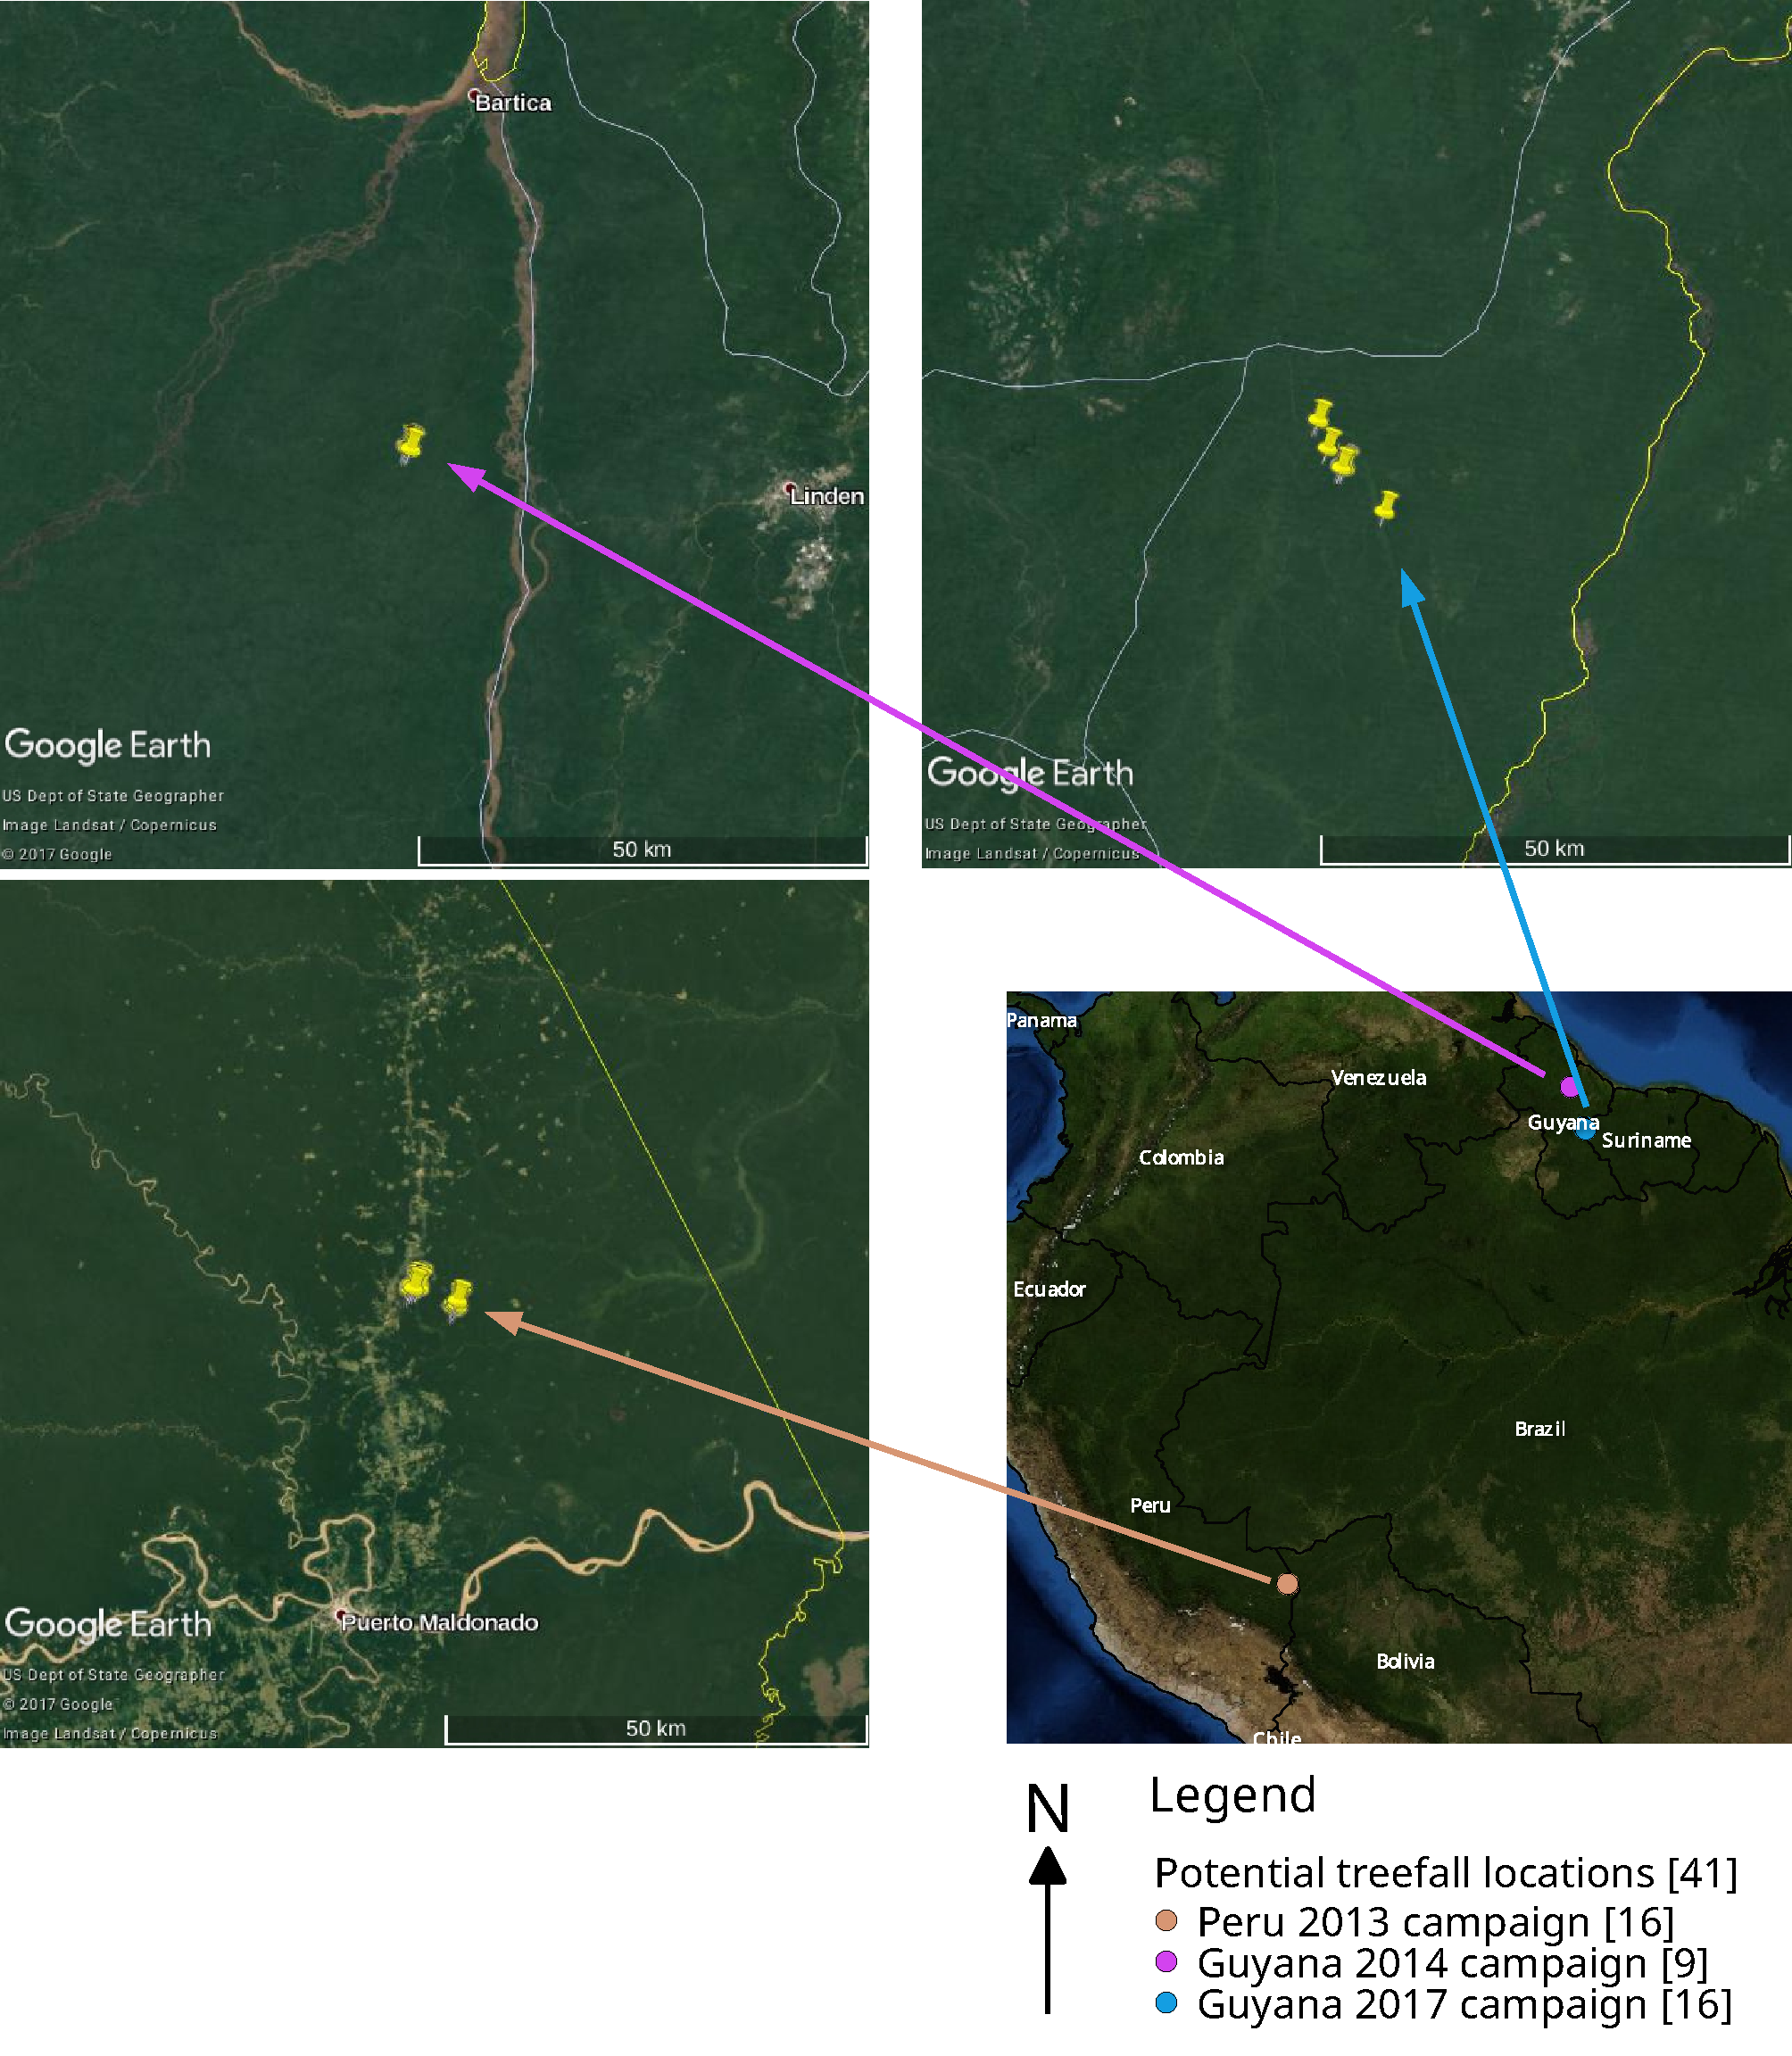
\includegraphics[width=\textwidth]{thesis-figures/17-all-sites-odg}
    \caption{Study sites with potential locations and numbers of selective logging treefall gaps, in the context of South America.}
    \label{fig-all-sites}
\end{figure}

\subsection{Peru, 2013}

The first field campaign was in November of 2013 in the Madre de Dios region of Peru. The selective logging operation took place in a forest east of the village Planchón, which is 37 km north of the region's capital city Puerto Maldonado. This region has a dry and a wet season, the latter spans from December to March. In the region, agricultural areas are encroaching upon previously intact forest \citep{scullion_assessing_2014}. Around Planchón, the agricultural fields are gradually expanding towards the forest from the Interoceanic Road that crosses Puerto Maldonado and goes through Planchón to Bolivia and Brazil.

The selective logging campaign was carried out by local villagers who obtained a permit for selective logging and harvesting of Brazil nuts (\textit{Bertholletia excelsa} Humb. \& Bonpl.) in a Brazil nut concession in a natural forest. The villagers did not have logging equipment such as skidders; instead, logs were processed on the spot using chainsaws, and the resulting planks were transported from the forest to the nearest road on tricycles. The larger trees in the study area have a canopy crown size of 20-30 m.

Nine trees to be cut down were scanned from 8 positions arranged in 30 by 50 m rectangles. The trees that were slated for logging were located on one end of the rectangle and were cut in a way so that they fall towards the middle of the plots. The location of each of the positions was determined using two separate Garmin \ac{GPS} devices. After logging, the same sites were scanned a second time. In this study, the centroid of all the measured points for each scanning site was used as a the approximate location of the treefall gaps. The scan dates both before and after logging were recorded. The actual logging event happened in between the two dates, which were between 2 and 6 days apart.

In addition to the logged tree data, there were also point locations of canopy gaps (seven in total) that are likely to have been the result of previously logged trees in the selective logging campaign (but may also have been created in earlier selective logging campaigns). In the case of gaps, only the post-logging date was recorded. In addition to \ac{GPS} data, there was also data on the nine main sites in a database, however, the locations did not match the locations measured by GPS. The entries in the database were offset from the GPS measurements by 540 metres to the north. Therefore in total 25 points from the Peru campaign were analysed for changes in reflectance following a selective logging event.

% TODO: Add image count statistics
% TODO: Add dates of selective logging
The area in which selective logging was known to take place was covered by Landsat images of path 2, rows 68 and 69. 731 Landsat 7 \ac{ETM+} images and 179 Landsat 8 \ac{OLI} images of this area were processed in this study.

\subsection{Guyana, 2014}

In both of the Guyana selective logging campaigns, logging was carried out by the Guyana Forestry Commission, a governmental organisation responsible for supervising forest concessions as well as granting and renewing logging permits in them. Lidar scanning was done as a research partnership between it and \ac{WUR} under the project \textit{SilvaCarbon}. The scans in these study sites were made by making plots of 30 by 40 m, and scanning from 13 positions. The trees were cut from a side towards the middle of the plot as well.% (funded by USAID): Measuring forest degradation for REDD+: a synthesis study across five SilvaCarbon countries.

The second field campaign took place in the east of the Cuyuni-Mazaruni region of Guyana in November 2014. The nine selectively logged trees that were scanned are located in the Wineperu concession of the Vairtana company, 40 kilometres south of the region's capital, Bartica. The town is connected to the selective logging sites by a road. The sites are very close to the road, 300 m away at most. Like the Peru campaign, the trees were scanned before and after the selective logging event. The area of selective logging was covered by Landsat images of path 231, row 56. In this study, 332 Landsat 7 \ac{ETM+} images of this area were processed in total.

\subsection{Guyana, 2017}

The third field campaign took place in the East Berbice-Corentyne region of Guyana in January 2017. The area where the trees were scanned is a very remote area at the end of a logging access road originally built in 1997 by the UNAMCO logging company, going south from the town of Kwakwani. After UNAMCO was closed in 2007, the road went unused until 2013, when the Ro-Anc company bought the concession and extended the road. For ease of timber extraction, a number of new primary logging roads (20 m across, gravel) were built in the logging site starting from 2014. Kwakwani is 85 kilometres north of the selective logging site.

In this campaign, a large number of inventoried trees were scanned, but trees were logged only in 16 of the locations. In some of these locations, clumps of more than one tree was inventoried and logged, with different heights and \ac{DBH}, up to a total of 26 trees. The \ac{DBH} class (20-40 cm, 40-60 cm, 60-80 cm, 80-100 cm and over 100 cm) of each tree was recorded. Some of the logged trees were relatively small (20-40 cm \ac{DBH}) and below the canopy of larger trees. In addition, no post-logging scans were made, so it is unknown when exactly the logging events happened. In this study it was assumed that the logging happened a similar time after the pre-logging scan as in the previous campaigns.

The area of selective logging was covered by the Sentinel-2 granules 21NUE and 21NUF, and Landsat tiles with paths 230 and 231, row 57. 185 Landsat 8 \ac{OLI} images and 70 Sentinel-2 \ac{MSI} images of this area were processed in total.

\section{Preprocessing workflow}

Satellite imagery of all the products used were available either in the Level 1C (top-of-atmosphere radiance) or Level 2A (top-of-canopy reflenctance) processing levels. For use with time series-based methods, this data had to be further preprocessed. All preprocessing of Level 2A data was done using the R programming language (version 3.3.1). A flowchart of the process is shown in figure \ref{fig-processing}.

\begin{figure}
  \centering
  \begin{tikzpicture}[node distance = 0.5cm, auto]
      \node [data] (l1amp) {Level 1C satellite imagery};
      \node [block, below= of l1amp] (atcor) {Atmospheric correction};
      \node [data, below= of atcor] (l2amp) {Level 2A satellite imagery};
      \node [block, below= of l2amp] (vi) {Vegetation index calculation};
      \node [block, below= of vi] (cloud) {Cloud masking};
      \node [block, below= of cloud] (mosaic) {Mosaicking, extent matching};
      \node [block, below= of mosaic] (stack) {Time series stacking};
      \node [block, below= of stack] (crop) {Cropping to bounding box};
      \node [block, right= of crop] (bbox) {Point bounding box calculation};
      \node [datasingle, above= of bbox] (ref) {Reference points};
      \node [block, below= of crop] (breaks) {Time series break detection};
      % Draw edges
      \path [line] (l1amp) -- (atcor);
      \path [line] (atcor) -- (l2amp);
      \path [line] (l2amp) -- (vi);
      \path [line] (ref) -- (bbox);
      \path [line] (vi) -- (cloud);
      \path [line] (bbox) -- (crop);
      \path [line] (cloud) -- (mosaic);
      \path [line] (mosaic) -- (stack);
      \path [line] (stack) -- (crop);
      \path [line] (crop) -- (breaks);
  \end{tikzpicture}
  \caption{Preprocessing chain. Grey blocks are input and output data, rounded blocks are scripts that process the data.}
  \label{fig-processing}
\end{figure}

\subsection{Top-of-canopy reflectance (Level 2A) processing}

Sentinel-2 imagery is currently made available as Level 1C products. These products were processed into Level 2A products by using the \texttt{sen2cor} software, version 2.3.1 \citep{mueller-wilm_sen2cor_2016}. \texttt{sen2cor} was set to use the 940 nm bands for water vapour correction, cirrus correction was enabled, a \ac{SRTM} \ac{DEM} was used for terrain correction and ozone column content data was set to be taken as best approximation from the metadata. All the other satellite imagery was already available in Level 2A and for those images this step was skipped.

\subsection{Vegetation index calculation}

For Sentinel-2 imagery, vegetation indices were calculated by using the formulae in section \ref{sec-vis}. In the case of \ac{NDMI} and \ac{NBR}, due to the lower spatial resolution of the \ac{SWIR} bands (20 m vs 10 m), the \ac{SWIR} bands had to be resampled to 10 m resolution by subdividing each pixel into four. Both nearest neighbour and bilinear interpolation resampling methods were tested.

For Landsat imagery, the vegetation indices were provided pre-calculated by \ac{ESPA}, so this step was also skipped.

In the case of \ac{ASTER} imagery, the post-2008 \ac{SWIR} bands are oversaturated, and the blue band is not captured by the \ac{ASTER} sensor, so only \ac{NDVI} and \ac{MSAVI} were calculated for this imagery.

\subsection{Cloud masking}

Clouds and cloud shadows had to be masked out from the satellite imagery in order to prevent spurious extremely high and low value observations in the time series. While some vegetation indices are insensitive to thin clouds and cloud shadows, all clouds and cloud shadows were masked in order to have consistent imagery for all vegetation indices in order to compare them. Masking involves replacing the reported reflectance values in cluded or shadowed areas of the images with \ac{NA} values.

% TODO: references for bfastSpatial
For Landsat data, clouds detected using the \texttt{Fmask} algorithm \citep{zhu_object-based_2012} and included in the pixel QA raster were masked out. Only pixels marked as clear (66 and 130 for \ac{ETM+}, 322 for \ac{OLI}) were kept, all other values were filtered out. This was done by using the R package \texttt{bfastSpatial} (development branch). In addition, values marked as oversaturated (reflectance values set to 20000) or fill (reflectance values set to -9999) in the reflectance images themselves were masked out as well.

For Sentinel-2 data, scene classification maps generated by \texttt{sen2cor} were used to mask out areas marked as no data, saturated, dark area, cloud shadows and all types of clouds.

\subsection{Mosaicking}

All of the study areas except for Guyana 2014 were located on the edge between two Landsat tiles or two Sentinel-2 granules. In order to make use of all the data available, tiles/granules from the same sensor taken at the same date were mosaicked together. Since the data that was mosaicked was in the form of vegetation indices, the rule applied when a pixel was covered by two images was to keep the higher pixel value of the two. This allows for filling in gaps left by masked out clouds and selecting the highest quality pixels. Since cloud shadows and clouds usually lower the value of vegetation indices, selecting higher values filters out the effects of clouds that were not detected (and thus not masked out in the cloud masking phase).

In addition to mosaicking, in this step all tiles were padded with \ac{NA} values in a way so that the extents of all images would match, in preparation for the time series stacking step.

\subsection{Time series stacking}

In order to make use of per-pixel vegetation index time series, all observations had to be stacked into one file with multiple layers, each layer representing one (potential) observation and containing information about the date of the observation. For Landsat data, this was done using the \texttt{bfastSpatial} package. For Sentinel-2 data, a script for stacking was created from scratch.

\subsection{Cropping to treefall gaps}

Tiles and granules cover a large area, whereas only the potential treefall gap areas were the focus of this study. In order to minimise the area to search through, images were cropped to the area around the treefall gap reference points. First, reference points were transformed into the \ac{UTM} projection that was used by the Landsat images of the area, then a buffer of 75 metre radius (150 metre diameter) was made around each point. Next, a bounding box of each buffer was calculated, and each time series stack was cropped to the bounding boxes. The result was one space-time cube per each reference treefall gap per each sensor. The spatial dimensions of the Landsat space-time cubes were 5 by 5 pixels, whereas Sentinel-2 spatial dimensions were 15 by 15 pixels.

\subsection{Time series analysis}

% TODO: Make BFAST into an acronym?
Lastly, pixels of the space-time cubes were analysed one by one by using the \texttt{BFAST} package \citep{verbesselt_detecting_2010} in order to attempt detection of selective logging treefall gaps. This is done by using trajectory analysis: a seasonal model is fit to the data by making use of known stable history prior to a logging event. Then, deviations from the values predicted by the model (residuals) are analysed at the time when a selective logging event potentially could have taken place. If the magnitude of observations exceeds a certain threshold, the first such observation is marked as a detected change.

In addition to treefall gaps, some nearby logging features such as logging roads and shifting cultivation were analysed with \texttt{BFAST} as well. The individual layers of the space-time cubes were also analysed visually, also in larger context and with comparison with higher resolution imagery from \ac{ASTER}, PlanetScope and DigitalGlobe imagery.

For Sentinel-2 \ac{MSI} imagery analysis, \texttt{BFAST} could not be used due to the lack of stable history to train the seasonal model on. The Sentinel-2A satellite started transmitting imagery in October of 2015; and due to frequent cloud cover over the Amazon the image time series is sparse, with too few observations to determine the natural variance of the vegetation indices. Instead, for this imagery, the pixels of the known treefall location space-time cubes were inspected for visible changes in the area. Pixels that showed changes in NDVI (44 in total) and NDMI (36 in total) were selected, and Welch's two-sample \textit{t}-test was used to determine whether the differences in the vegetation index values before and after logging are significant, as well as to compare the estimated true means of each vegetation index before and after logging.

\chapter{Results}

\section{Logging feature detectability}

\subsection{Treefall gaps, skid trails}

% Automation possibilities, pictures of areas, some telling time series examples, Landsat-to-Sentinel comparison

\subsubsection{Sentinel-2}
\label{sec-treefall-sentinel2}

\begin{figure}
  \centering
  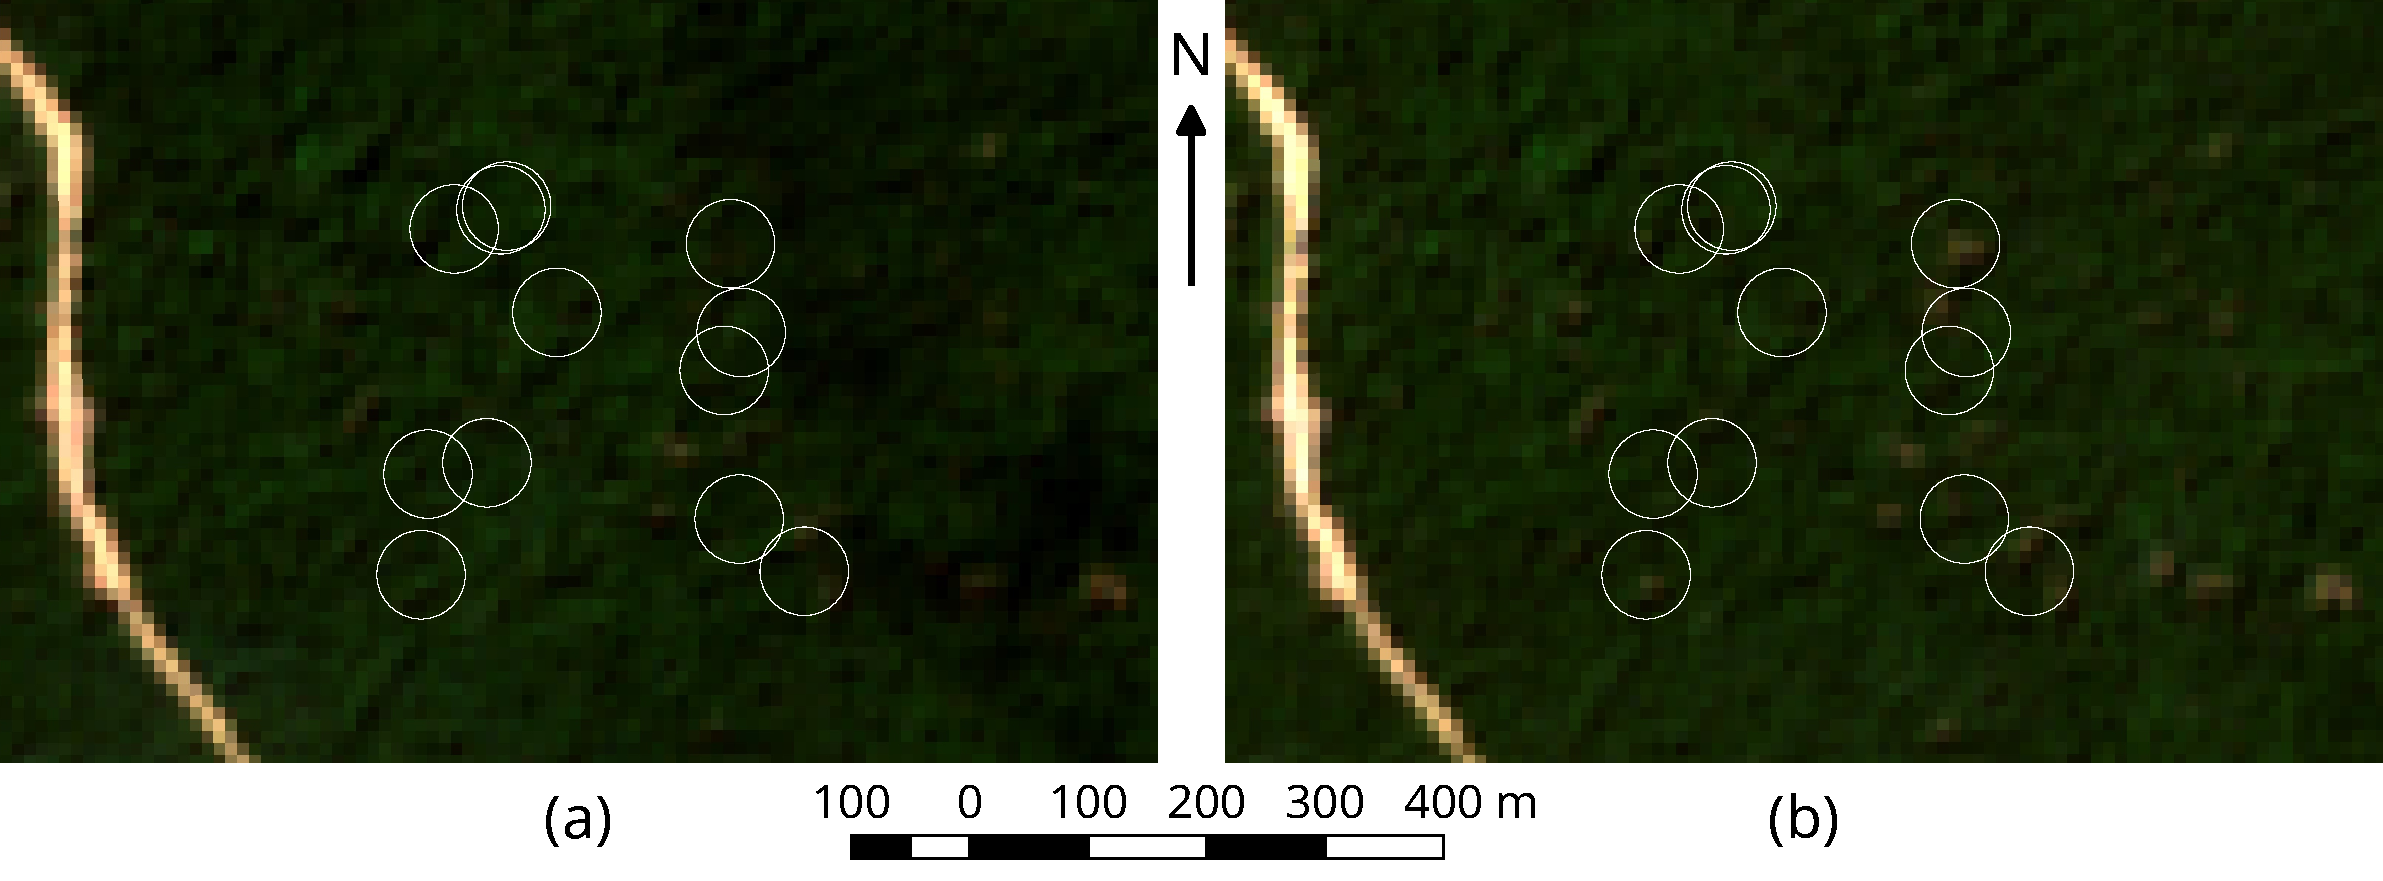
\includegraphics[width=\textwidth]{thesis-figures/02-guyana-sentinel2-tci}
  \caption{Sentinel-2 \ac{MSI} true colour image subset from the Guyana 2017 study site. White circles indicate the 75 m radius around known logging locations. (a): site prior to known selective logging (January 13, 2017). The dark parts on the right are cloud shadows. (b): site after known selective logging (February 12, 2017).}
  \label{fig-guyana-sentinel2-tci}
\end{figure}

\begin{figure}
  \centering
  \begin{subfigure}[b]{0.32\textwidth}
    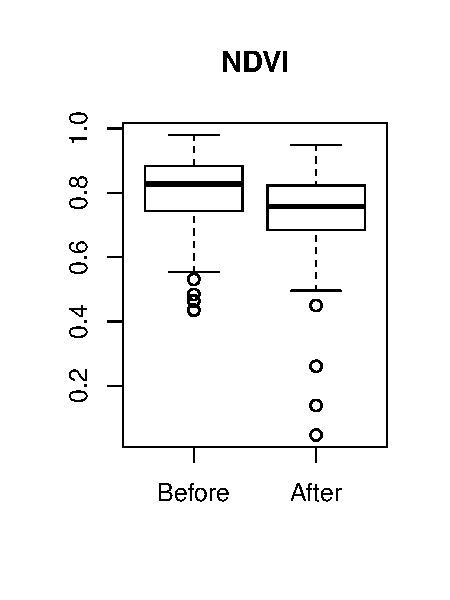
\includegraphics[width=\textwidth]{thesis-figures/03-boxplot-ndvi}
  \end{subfigure}
  \begin{subfigure}[b]{0.32\textwidth}
    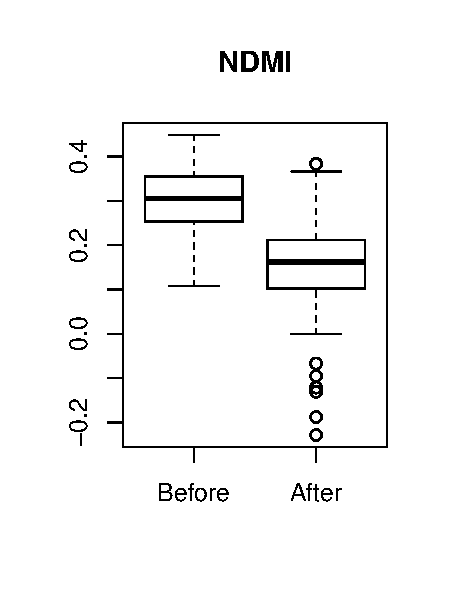
\includegraphics[width=\textwidth]{thesis-figures/04-boxplot-ndmi}
  \end{subfigure}
  \begin{subfigure}[b]{0.32\textwidth}
    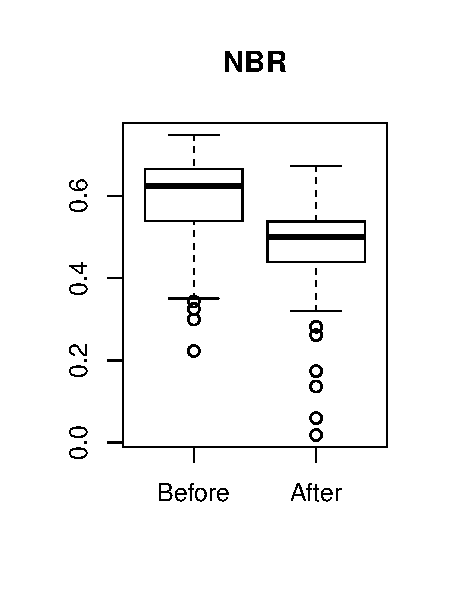
\includegraphics[width=\textwidth]{thesis-figures/05-boxplot-nbr}
  \end{subfigure}
  \begin{subfigure}[b]{0.32\textwidth}
    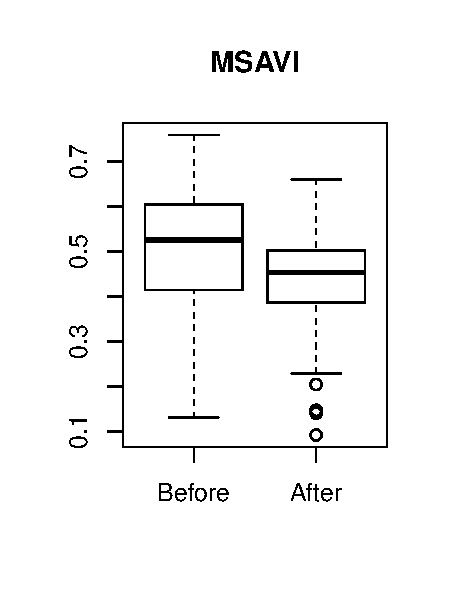
\includegraphics[width=\textwidth]{thesis-figures/06-boxplot-msavi}
  \end{subfigure}
  \begin{subfigure}[b]{0.32\textwidth}
    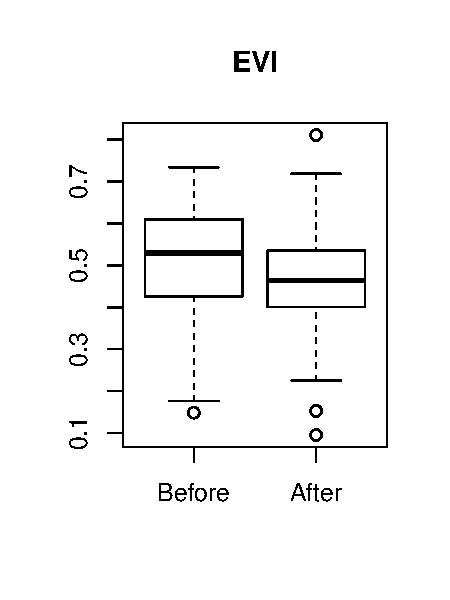
\includegraphics[width=\textwidth]{thesis-figures/07-boxplot-evi}
  \end{subfigure}
  \caption{Distribution of vegetation index values before and after the known logging event in affected Sentinel-2 \ac{MSI} pixels. The bold line in the middle represents the median, the hinges of the box represent the 1st and 3rd quartiles, and the whiskers represent 1.5 of the interquartile range, circles are outliers.}
  \label{fig-boxplots}
\end{figure}

\begin{table}
  \resizebox{\textwidth}{!}{
    \begin{tabular}{p{2.5cm}p{2.3cm}p{3.3cm}p{3.3cm}p{3.3cm}p{3.5cm}}
    Study site and year & Potential gap locations & Known logged trees & Logged trees with known logging date & Identified gaps (low confidence) & Identified gaps (high confidence)\\
    \hline
    Peru, 2013 & 25 & 16 & 9 & 1 & 0\\
    Guyana, 2014 & 9 & 9 & 9 & 4 & 0\\
    Guyana, 2017 & 16 & 16 & 0 & 9 & 7
    \end{tabular}
  }
    \caption{Summary of known logged tree locations and identified treefall gaps. Trees with known logging date are trees with records of dates both before and after logging (the others were missing either one of the two dates). High confidence for gap identification means that at least two vegetation indices indicated a change and the change was persistent at least in two subsequent images right after the logging date.}
    \label{tab-tree-count}
\end{table}

% TODO: Expand this example: either add NDVI or a control pixel or Landsat: NDVI and control is a good idea
\begin{figure}
  \centering
  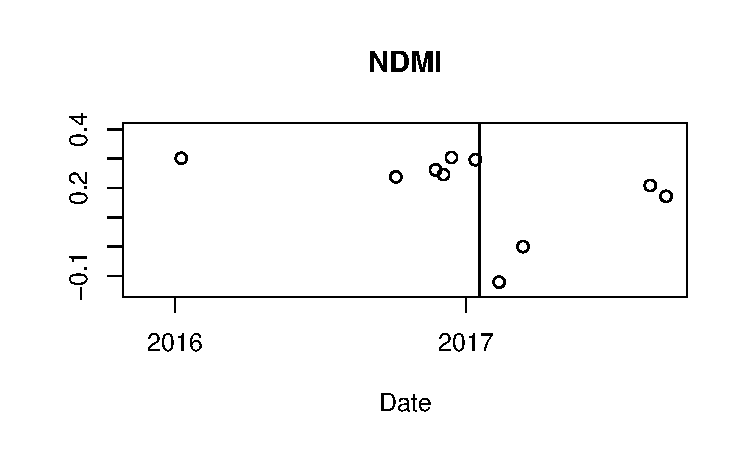
\includegraphics[width=0.6\textwidth]{thesis-figures/08-guyana-ts-ndmi}
  \caption{A time series of all Sentinel-2-derived \ac{NDMI} values for an example pixel where a treefall gap appeared. The vertical line indicates the date after which the selective logging event happened.}
  \label{fig-guyana-ts-ndmi}
\end{figure}

In the Guyana 2017 study area, from the 16 reference points of known logged trees, only 9 treefall gaps could be identified using Sentinel-2 imagery, and only 7 of them with confidence (see table \ref{tab-tree-count} and figure \ref{fig-guyana-sentinel2-tci}). Two of the reference points were within a 6 m distance from one another, which made them not distinct from one another. In the other cases where the gap was not visible, an existing gap, logging road or log deck was nearby. In the case there is an existing logging gap, according to \ac{RIL} conventions the tree should be felled in the direction of the gap in order to minimise canopy damage.

% TODO: Write about t-tests and controls in methods
\begin{table}
  \resizebox{\textwidth}{!}{
    \begin{tabular}{llllllll}
    Vegetation index & Mean before logging & Mean after logging & Change magnitude & $p$-value\\
    \hline
    NDVI in affected pixels & 0.798±0.014 & 0.743±0.020 & -0.055±0.024 & <0.001\\
    NDMI in affected pixels & 0.300±0.010 & 0.150±0.017 & -0.150±0.019 & <0.001\\
    NBR in affected pixels & 0.599±0.012 & 0.481±0.017 & -0.118±0.021 & <0.001\\
    MSAVI in affected pixels & 0.494±0.020 & 0.438±0.017 & -0.056±0.026 & <0.001\\
    EVI in affected pixels & 0.504±0.019 & 0.463±0.019 & -0.041±0.027 & 0.003\\
    \hline
    NDVI control & 0.819±0.017 & 0.840±0.020 & 0.021±0.026 & 0.117\\
    NDMI control & 0.306±0.011 & 0.289±0.012 & -0.018±0.016 & 0.036\\
    NBR control & 0.611±0.013 & 0.601±0.014 & -0.009±0.019 & 0.338\\
    MSAVI control & 0.524±0.016 & 0.583±0.018 & 0.059±0.024 & <0.001\\
    EVI control & 0.525±0.015 & 0.588±0.016 & 0.063±0.022 & <0.001
    \end{tabular}
  }
  \caption{Change in vegetation index magnitude after a known logging event in the Guyana 2017 study area. Affected pixels are contiguous pixels with visually apparent change less than 75 m away from the location of known logged trees, control are four pixels 106 m away from each location of a known logged tree. Errors are 95\% confidence intervals.}
  \label{tab-vi-magnitudes}
\end{table}


Of the treefall gaps that were visible, on average the changes affected 5 pixels (500 m² area) in NDVI and 4 pixels (400 m² area) in NDMI. The values of each vegetation index tested were significantly ($ p < 0.003 $) lower after logging than before it (see table \ref{tab-vi-magnitudes} and figure \ref{fig-boxplots}). See figure \ref{fig-guyana-ts-ndmi} for an example of how the time series of one treefall gap pixel looks like.

\begin{figure}
  \centering
  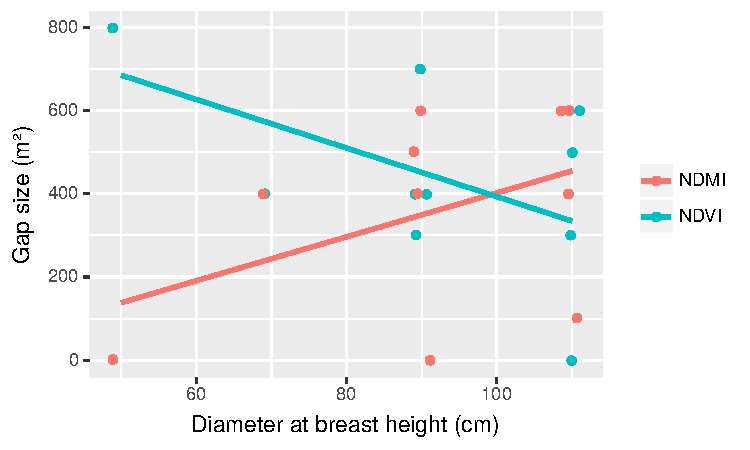
\includegraphics{thesis-figures/18-gap-vs-dbh}
  \caption{Regressions between the apparent gap size and the \ac{DBH} of the largest tree logged at the location of each gap, grouped by vegetation index. The points are jittered to avoid overplotting. Precision of \ac{DBH} is 20 cm, precision of gap size is 100 m², sample size is 10 gaps.}
  \label{fig-gap-vs-dbh}
\end{figure}


The correlations between the visible gap size and the \ac{DBH} of the logged tree were insignificant in both NDVI ($r^2=0.26$, $p=0.13$) and NDMI ($r^2=0.19$, $p=0.21$), see figure \ref{fig-gap-vs-dbh}.

\subsubsection{Landsat imagery}

\begin{figure}
  \begin{subfigure}{\textwidth}
    \centering
    \includegraphics[width=0.75\textwidth]{thesis-figures/09-guyana17-landsat-ndmi-undetected}
  \end{subfigure}
  \begin{subfigure}{\textwidth}
    \centering
    \includegraphics[width=0.75\textwidth]{thesis-figures/10-guyana17-landsat-ndmi-detected}
  \end{subfigure}
  
  \caption{\texttt{BFAST} Monitor analysis of an \ac{NDMI} time series for two Landsat 8 \ac{OLI} pixels where treefall gaps are visible in Sentinel-2 \ac{MSI} imagery of the same areas. Top: no change is detected due to too low magnitude of change, and some unfiltered clouded pixels in the history period. Bottom: change is detected successfully.}
  \label{fig-guyana17-landsat-ndmi}
\end{figure}

In Landsat imagery of the Guyana 2017 study area, only 3 gaps within the vicinity of the known logged trees could be identified. The rest were not visible either due to cloud cover in Landsat scenes, or due to pixel border effects: gap centre going through the boundary of 2 or 4 pixels, therefore dispersing the signal into several pixels. That makes the treefall gaps unidentifiable due to a low signal-to-noise ratio. The gaps that can be identified in Landsat imagery also show a smaller magnitude of change due to the larger area covered by each pixel (900 m² compared to 100 m² in Sentinel-2 \ac{MSI}).

\texttt{BFAST} analysis of Landsat imagery in the Guyana 2017 study site yielded only a single detection of a treefall gap, and only when using \ac{NDMI}. The other two gaps, while visible when inspecting the time-space cube (the value of the pixel changes compared to the surroundings), are not detected by \texttt{BFAST} due to the low magnitude of change (see figure \ref{fig-guyana17-landsat-ndmi}).

\texttt{BFAST} was not able to detect any treefall gaps in other study sites. In the case of Landsat 8 \ac{OLI} imagery of the Guyana 2014 site, a lot of false positives were generated due to too few observations in stable history (which was a period of less than one year). When using Landsat 7 \ac{ETM+} imagery of the same areas, no breaks were detected.

Skid trails were not visible from any of the satellite imagery used, in any of the study sites. In \ac{RIL}, skid trails are planned in advance in a way that minimises the damage done, which means that there are no changes to the top of canopy that would be visible from satellite imagery.

% Which sensors can be used with BFAST due to history, what are the effects of the resolution

\subsubsection{ASTER}

% TODO: Add some reference images?

\ac{ASTER} imagery of all the study sites were useful for better visualisation of the forest structure and the effects of forest features to vegetation index values, due to the finer pixel size compared to Landsat. However, the combination of a long revisit time and frequent cloud cover resulted in only one or two usable images per year, which is not enough for neither time-series-based analysis nor statistical analysis. At 15 m resolution, individual trees cannot be visually picked out unless they stand apart from other trees or have a different seasonal cycle compared to neighbouring trees.

Another limiting factor of \ac{ASTER} imagery is the range of digital numbers. Whereas Landsat and Sentinel-2 use the range of 0-10000 for digital numbers of each band, \ac{ASTER} uses the range of 0-1000. This affects the range of derived vegetation index values: the smallest step between two values is 0.005. Any value in between is clamped to one or the other side and may not be distinguishable from the surroundings if neighbouring trees have similar values, which happens at the higher end of vegetation index saturation.

\subsection{Clearcut areas, logging roads, log decks}

\begin{figure}
  \begin{subfigure}{\textwidth}
    \centering
    \includegraphics[width=0.75\textwidth]{thesis-figures/11-guyana17-landsat-ndvi-deck}
  \end{subfigure}
  \begin{subfigure}{\textwidth}
    \centering
    \includegraphics[width=0.75\textwidth]{thesis-figures/12-guyana17-landsat-ndvi-road}
  \end{subfigure}
  \caption{\texttt{BFAST} Monitor analysis of Landsat 8 \ac{OLI} \ac{NDVI} time series in the Guyana 2017 study site. Top: the central pixel of a log deck built in 2016. Bottom: a pixel on a road built in 2014. The increase visible in 2016 is due to the shifting of the road one pixel to the north in that image, which could be due to georeferencing issues or different sun-sensor angle.}
  \label{fig-guyana17-landsat-ndvi-deck}
\end{figure}

Larger-scale disturbances associated with selective logging, such as major logging roads as well as clearcuts or slash-and-burn activities, were detectable from both Landsat and Sentinel-2 imagery. Given sufficient historical data, \texttt{BFAST} was able to automatically detect such disturbances and determine the approximate time at which they happened, using any of the tested vegetation indices (see figure \ref{fig-guyana17-landsat-ndvi-deck}).

\begin{figure}
  \begin{subfigure}{\textwidth}
    \centering
    \includegraphics[width=\textwidth]{thesis-figures/13-peru-shifting}
  \end{subfigure}
  \begin{subfigure}{\textwidth}
    \centering
    \includegraphics[width=\textwidth]{thesis-figures/14-peru-shifting-ndvi}
  \end{subfigure}
  \caption{Landsat 7 \ac{ETM+} time series of a pixel in a shifting cultivation plot in the Peru study site. Top: \ac{NDMI}. Several disturbance and regrowth cycles are visible and the first one is detected by \texttt{BFAST} Monitor. Bottom: \ac{NDVI}. Only the largest disturbance is visible and is detected, but the \ac{NDVI} values after the disturbance are higher than before it.}
  \label{fig-peru-shifting-cultivation}
\end{figure}

However, the presence of these disturbances varied greatly across the different study sites: in Peru and Guyana 2014, the selective logging campaigns were carried out close to an existing road, therefore no additional disturbances that would indicate that selective logging had occurred appeared in that area. In Guyana 2017, logging roads and log decks were built specifically for facilitating the selective logging campaign, some of them several years in advance (see figure \ref{fig-guyana17-landsat-ndvi-deck}). The Peru study site was the only one where land use was being changed from forest to shifting cultivation or rangelands, next to the selective logging site. The Landsat time series in that area was unique, with multiple points of disturbance spaced out over several years (see figure \ref{fig-peru-shifting-cultivation}, top). The \ac{NDVI} values after a clearcut go down quickly, and take a year to recover to their pre-disturbance values; after that point, \ac{NDVI} values exceed those of the original undisturbed forest (see figure \ref{fig-peru-shifting-cultivation}, bottom).

\section{Vegetation index comparison}

% Sensitivity, threshold values, correlation, images at small scale and large scale
For treefall gap detection, as discussed in section \ref{sec-treefall-sentinel2}, there were significant differences in means before and after a selective logging event in all of the tested vegetation indices. However, the magnitude of change differed (see figure \ref{fig-boxplots}), and so did the ability to detect larger logging features (see figure \ref{fig-peru-shifting-cultivation}).

\subsection{NDVI}

\ac{NDVI} was found to be less sensitive to changes in forest structure than the other vegetation indices tested; on average NDVI values in pixels affected by selective logging decreased from 0.80 to 0.74. Changes in \ac{NDVI} are also dependent on the forest floor in the particular area: if the forest floor under the logged tree consisted of photosynthetic vegetation, the change in NDVI was small, or even positive (see figure \ref{fig-peru-shifting-cultivation}). In contrast, if the forest floor consisted mainly of non-photosynthetic vegetation or bare soil, or if the forest floor was damaged, \ac{NDVI} was a reliable indicator of treefall gaps and other logging features (see figure \ref{fig-guyana17-landsat-ndvi-deck}).

% TODO: Add ASTER/Landsat/Sentinel-2 image of NDVI, where it really matters
One unique property of \ac{NDVI} was found to be its relation to shadows. Since \ac{NDVI} is a ratio of the reflectance in the red band and the reflectance in the \ac{NIR} band, when vegetation is shadowed (e.g. by a cloud shadow), the reflectance in red becomes close to 0 and thus \ac{NDVI} becomes close to 1. On the other hand, the reflectance in \ac{NIR}, and thus \ac{NDVI}, may be lower in forests compared to grasslands due to the complex canopy structure (however, this varies seasonally due to leaf flush). The result of both of these properties combined is that grasslands and forests have differing \ac{NDVI} values, and cloud shadows and tree shadows over photosynthetic vegetation appear brighter compared to unshadowed area and tree canopies, respectively.

\subsection{NDMI, NBR}

The \ac{SWIR}-based vegetation indices \ac{NDMI} and \ac{NBR} were the most sensitive to changes in forest structure from all the vegetation indices tested, as seen in figure \ref{fig-boxplots}. After a logging event, mean \ac{NDMI} values in affected pixels decreased from 0.30 to 0.15, whereas \ac{NBR} values decreased from 0.60 to 0.48. The relative magnitude of change was higher in \ac{NDMI} than in \ac{NBR}. \ac{NDMI} values differ more within forests, revealing their structure, whereas \ac{NBR} tends to vary less within forests but highlight only particularly large disturbances. However, the two indices are highly correlated with one another (Pearson's correlation: 0.94), as the only difference between them is the choice of the \ac{SWIR} wavelength.

The \ac{SWIR}-based indices turned out to be highly sensitive to internal shadows within forests, but insensitive to cloud shadows, because unlike the red band, \ac{NIR} values are higher than zero when a cloud shadow is over vegetation, and cloud shadows reduce the reflectance in \ac{NIR} and \ac{SWIR} almost equally. This is a useful property, because it allows the use of pixels that for other vegetation indices would not be useful, and it also helps when the cloud shadow masks are not perfectly reliable (as is often the case). Sensitivity to internal shadows comes from the \ac{NIR} band, whereas the \ac{SWIR} band is smooth and does not capture internal shadows, but is good at capturing the high reflectance from bare soils.

One issue of calculating \ac{NDMI} and \ac{NBR} is that the \ac{SWIR} band often times has a coarser resolution than the visible and \ac{NIR} bands due to lower amounts of energy returned from the land surface at those wavelengths. This is the case in Sentinel-2 and \ac{ASTER} imagery. Therefore in order not to lose information from the \ac{NIR} band, the \ac{SWIR} band data has to be upsampled to match the \ac{NIR} band pixels. This can be done by using nearest neighbour interpolation or bilinear interpolation. Testing of both interpolation methods revealed that in forests, nearest neighbour resampling leads to block artefacts and could be misleading, whereas bilinear interpolation was more appropriate, however the differences are overall small for gaps. The largest differences were within logging roads, where the road outlines would become blurred when using bilinear interpolation and blocky in a salt-and-pepper pattern when using nearest neighbour interpolation.

\subsection{EVI, MSAVI}

The other two vegetation indices tested, \ac{EVI} and \ac{MSAVI}, are both complex indices that were designed to overcome the deficiencies in \ac{NDVI}. Even though the approaches differ, the result is largely the same: both vegetation indices are highly correlated in forests (Pearson's correlation: 0.94). The two indices are in between \ac{NDVI} and the \ac{SWIR}-based indices in sensitivity: they capture bare soils and non-photosynthetic vegetation like \ac{NDVI} does, and are sensitive to internal shadowing like the \ac{SWIR}-based indices. However, they are less sensitive to either compared to the other types of vegetation indices, thus the overall sensitivity to selective logging events is rather poor (see figure \ref{fig-boxplots}).

\ac{EVI} is unique in that it compensates for the presence of thin clouds and cloud edges. This is a useful property, since while most cloud masking approaches are good at detecting thick clouds, thin ones are much more difficult to detect. However, unlike the \ac{SWIR}-based indices, \ac{EVI} is affected by the presence of cloud shadows. \ac{EVI} was also the vegetation index that is least correlated with any of the others except \ac{MSAVI}: 0.68 correlation with \ac{NDMI} and 0.69 correlation with \ac{NDVI} and \ac{NBR}.

\ac{MSAVI} is highly correlated with \ac{EVI}, and the main difference between the two is that \ac{MSAVI} does not share the property of atmospheric noise correction and thus is affected by light clouds. On the other hand, only the red and \ac{NIR} bands are required to calculate \ac{MSAVI}, whereas \ac{EVI} also requires the blue band, which is not always captured (e.g. by \ac{ASTER}).

\chapter{Discussion}

\section{Selective logging detection possibilities}

% What is possible to detect, in a case study format; this should answer the first research question

The results showed that the ability to detect selective logging treefall gaps from Landsat imagery is extremely limited, which confirms the findings of \citet{asner_remote_2002} and \citet{asner_canopy_2004}. Even when the location and appearance time of the canopy gap is known, the 30 m resolution of Landsat is not enough to reliably detect changes, neither in an automated way nor manually. While the tree canopy size in the Amazon rainforest tends to reach 30 m in diameter, it is very rare that the pixel grid would align with the gap left by logging a particular tree. The more common case is for the gap to be split into two or four pixels, in which case the effect that the logging event has to vegetation index values are too low due to the influence of the surrounding untouched vegetation.

However, the results showed that the 10 m resolution of Sentinel-2 \ac{MSI} is enough to visually detect most treefall gaps, and that it should be possible to detect the gaps in an automated way in the future, when Sentinel-2 imagery time series grow in length so as to allow using time-series-based detection methods.

From the other selective logging features identified by \citet{asner_remote_2002}, skid trails were not identifiable from any of the satellite imagery used, whereas large logging roads and log decks were both identifiable and automatically detectable from both Landsat and Sentinel-2 imagery. These findings are similar to those of \citet{read_spatial_2003}.

% TODO: Could make it into an enumerate list; the rest of the information can go into the VI section
An analysis of detected logging features follows.

\begin{figure}
  \centering
  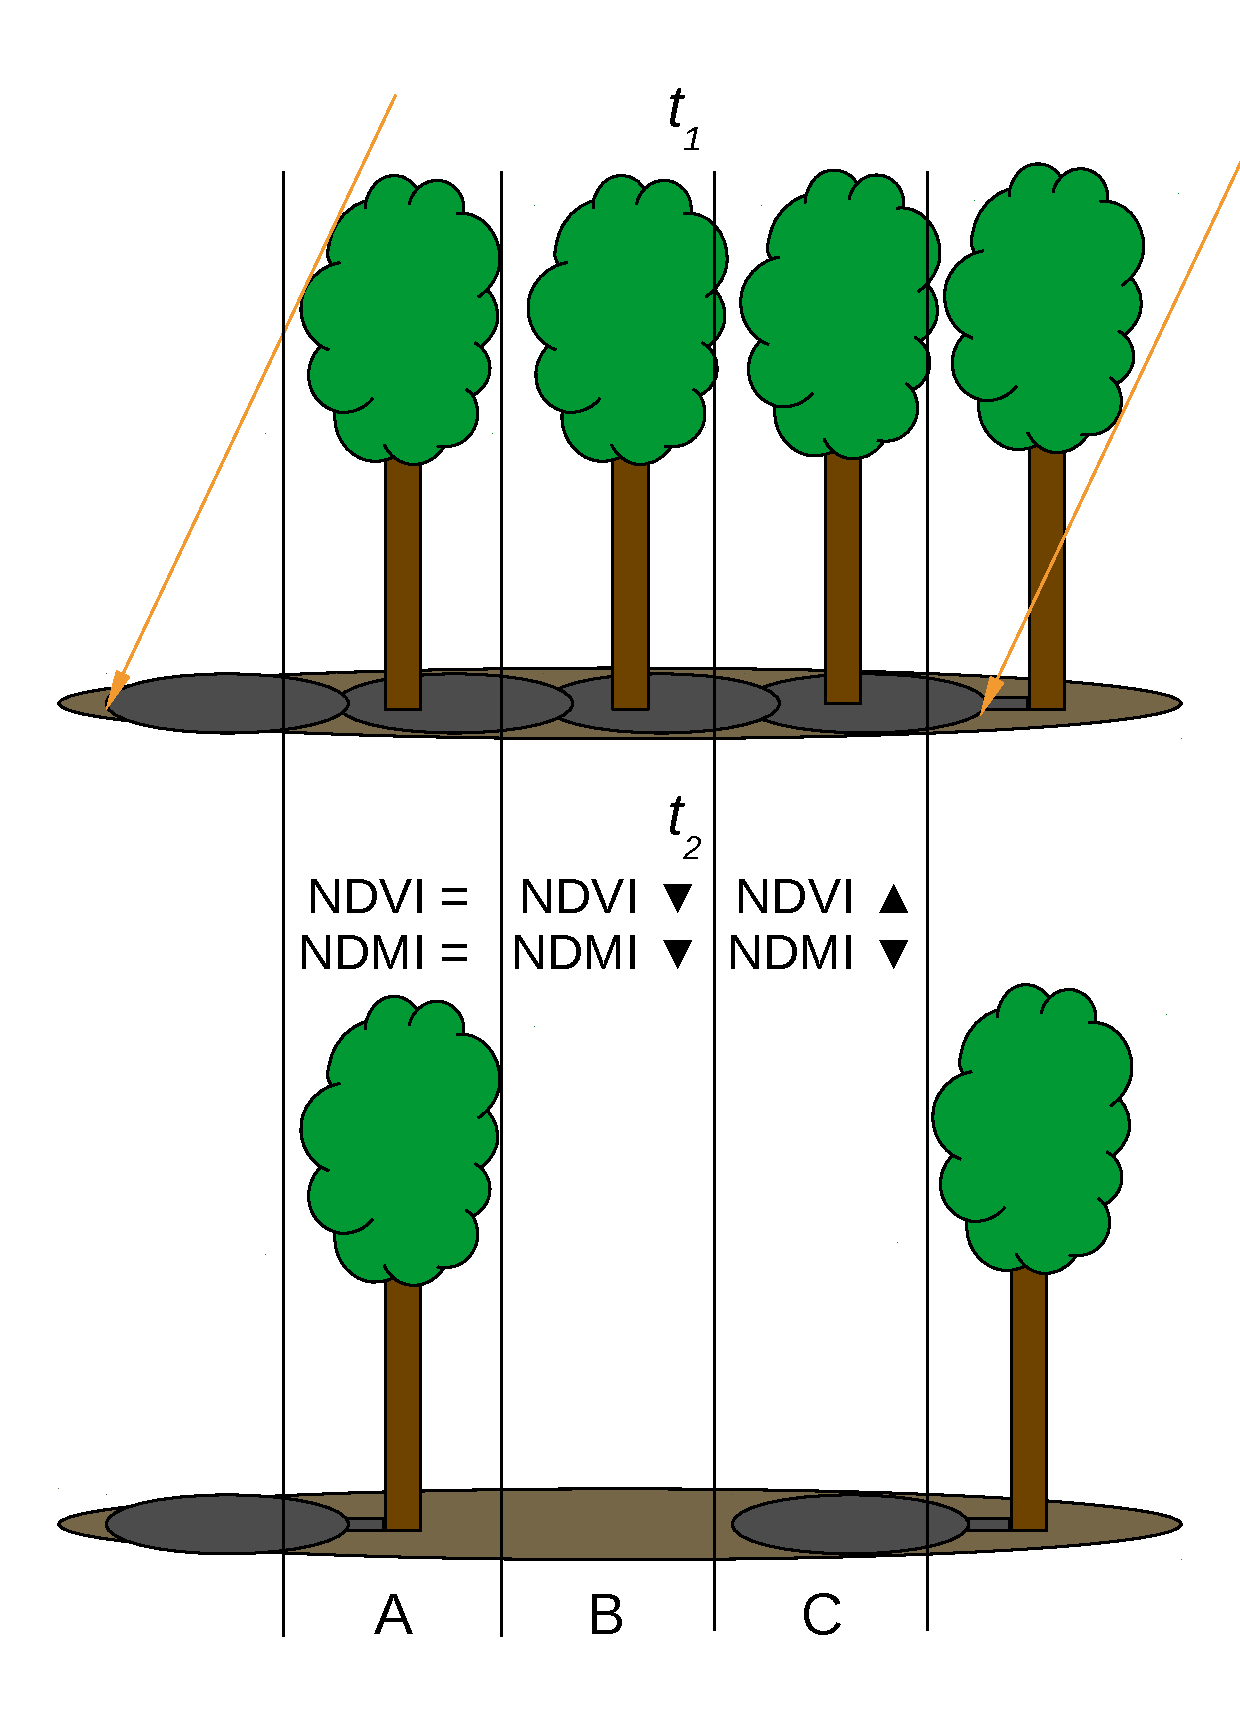
\includegraphics[width=0.5\textwidth]{thesis-figures/15-gap-vi-model}
  \caption{A simple theoretical 2D model of changes in vegetation indices in a forest following selective logging of two trees. Orange arrows indicate the sun incidence angle, black lines indicate pixel boundaries of a nadir-facing satellite sensor. At timestep $ t_{1} $ all three pixels have high \ac{NDVI} and \ac{NDMI} values. After logging at timestep $ t_{2} $, pixel A has high \ac{NDVI} and \ac{NDMI}, pixel B has low \ac{NDVI} and \ac{NDMI}, pixel C has high \ac{NDVI} but low \ac{NDMI} values. In case of a smaller gap, pixel B would have the same values as pixel A, and so \ac{NDVI} would not be useful for gap identification.}
  \label{fig-gap-vi-model}
\end{figure}

\subsection{Moderate size gaps in dense forests with a soil background}

% Case of Guyana 2017: cutting down a tree makes soil appear, visible in \ac{NDVI}

If the forest floor is bare soil or non-photosynthetic vegetation, as in Guyana 2017 study site, then the treefall gaps are identifiable by a change in \ac{NDVI} (see figure \ref{fig-gap-vi-model}, B). This is due to photosynthetic vegetation strongly absorbing light in the red band and strongly reflecting light in the \ac{NIR} band.

% TODO: can add an image of NDVI
These types of gaps are also discernable visually by inspecting the \ac{NDVI} values, as fresh treefall gaps are small and thus stand out from intact forest. However, they do not stay visible for long due to canopy and forest floor regrowth.

\subsection{Small gaps in dense forests}

% Case of Guyana 2017: cutting down a tree results in a shift in shadows, visible in \ac{NDMI}

If the treefall gaps are too small to cover a pixel size area, or if the forest floor is vegetated, the gaps can still be identified indirectly using \ac{NDMI} due to a shift in the forest texture, as new internal shadows from nearby trees appear on the edges of the newly created gap (see figure \ref{fig-gap-vi-model}, C). This allows for identifying selective logging of smaller trees, however, it is an indirect indicator of gaps. Shadows may also shift due to sun-sensor angle geometry, potentially confounding automated detection algorithms.

\subsection{Logging roads}

Case of Guyana 2017: logging roads are easy to detect, but not skid trails. In other cases logging roads are not detected either (only skid trails used/under canopy/too narrow)

\subsection{Clear-cuts}

% Case of Peru 2013: clear-cuts highly affect \ac{NDVI} for a year, followed by an increase in \ac{NDVI} compared to the beginning due to less shadowing

When deforestation happens as part of slash-and-burn agriculture or shifting cultivation, as the case was in the Peru study site, it can be identified using methods based on time series in an automated way. Since the area that is affected is large, Landsat imagery can be used for this purpose, and its long archive is andvantageous in that case. In case of tree plantations or shifting cultivation, this method can be used to determine the time it takes for the canopy to regrow and reach pre-harvest levels, though the estimates depend on how fast the vegetation index used saturates (see figure \ref{fig-peru-shifting-cultivation}). However, this type of logging is already relatively well-understood and is not usually considered to be selective logging.

% In \ac{NDVI} the post-harvest values may become higher than pre-harvest ones due to 

\section{Comparison of vegetation indices}

Of the five vegetation indices tested (\ac{NDVI}, \ac{NDMI}, \ac{NBR}, \ac{EVI}, \ac{MSAVI}), three groups were identified according to how the indices perform in forests and what changes are evident when a selective logging event occurs. No one index is best for detecting selective logging, and a combination of several indices may be advantageous for detection purposes.

\subsection{NDVI}

\begin{figure}
  \centering
  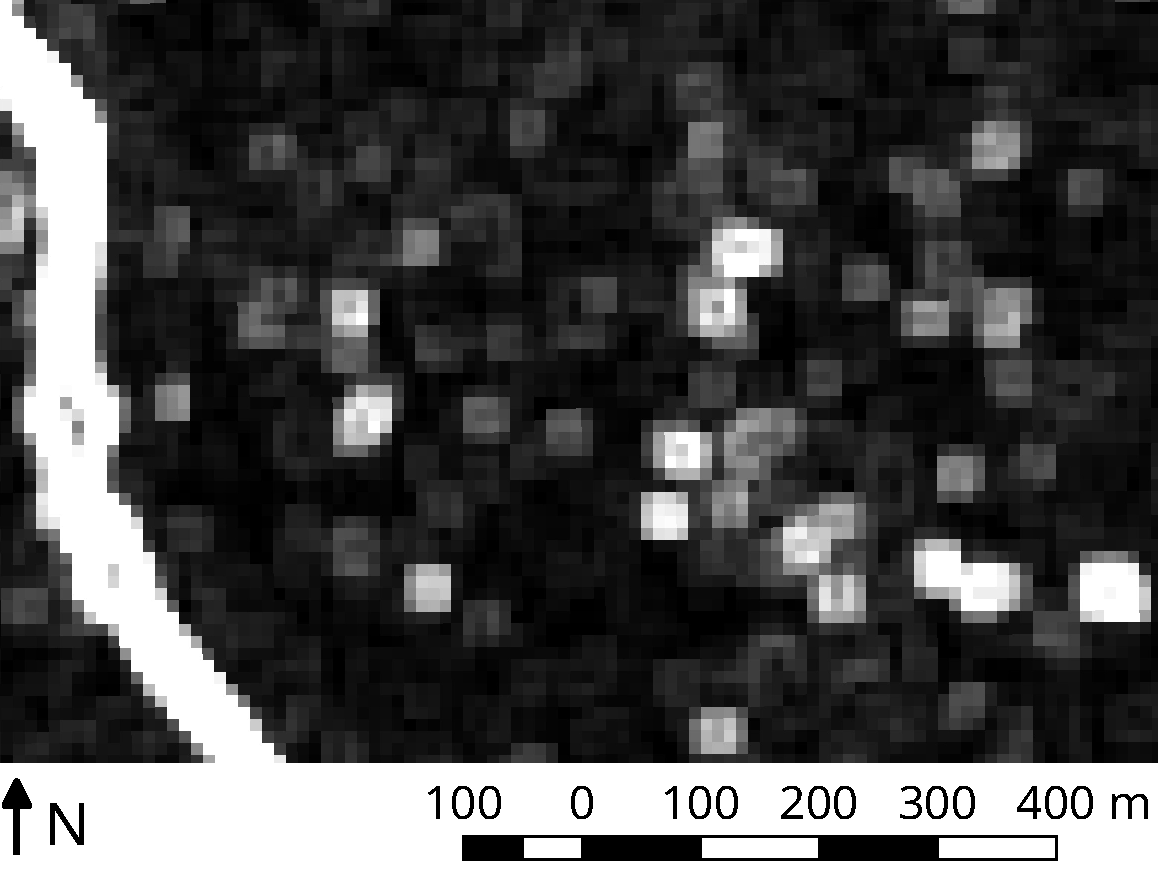
\includegraphics[width=0.5\textwidth]{thesis-figures/16-guyana17-ndvi-texture}
  \caption{Texture analysis of the Guyana 2017 study site Sentinel-2 image of February 12. Black corresponds to a standard devation in \ac{NDVI} of 0.0044, white to 0.0921 in a 3 by 3 pixel moving window.}
  \label{fig-ndvi-texture}
\end{figure}

\ac{NDVI} was unlike other vegetation indices tested in that shadows cause high rather than low values of the vegetation index. This makes \ac{NDVI} especially useful for initial detection of selective logging treefall gaps. As long as the background behind the canopy is non-photosynthetic and the gap size compared to sensor spatial resolution allows for it, gaps in \ac{NDVI} stand out clearly from the surroundings. Forests appear rather homogeneous in \ac{NDVI}, since internal shadowing causes an increase in \ac{NDVI}, but a small one, since \ac{NDVI} is close to saturation (0.85-0.95) in forests in the first place. A gap with a soil background visible causes a marked decrease in \ac{NDVI}.

One possible application for \ac{NDVI} in treefall gap detection would be in spatial texture analysis. \citet{asner_remote_2002} used variance in a 3 by 3 pixel moving window on Landsat \ac{ETM+} imagery as an indicator of texture, and while it did not result in useful detection of treefall gaps, it could be useful in combination with Sentinel-2 \ac{MSI} imagery (see figure \ref{fig-ndvi-texture}, cf. figure \ref{fig-guyana-sentinel2-tci}). There is a number of spatial texture analysis methods, such as the median above 90th percentile used by \citet{hamunyela_using_2016}, and more research is needed to determine the most appropriate method specifically for treefall gap detection.

\subsection{NDMI, NBR}

While \ac{NBR} is a highly popular index for logging detection \citep{shimizu_using_2017, schneibel_assessment_2017}, the related \ac{NDMI} had a more pronounced change in values after a selective logging event, the most of all indices tested (see figure \ref{fig-boxplots}). Thus \ac{NDMI} is the most useful single vegetation index for detecting selective logging events of all the ones tested in this study.

Furthermore, neither \ac{NDMI} nor \ac{NBR} are affected by cloud shadows, therefore more data can be used. \ac{NDMI} is also less affected by thin clouds compared to other indices, with the exception of \ac{EVI}. This is a major advantage in the Amazon region, where cloud cover if frequent, and is also useful in the cases when the built-in cloud and cloud shadow detection algorithms for satellite imagery products fail to detect thin clouds and cloud shadows properly.

However, while \ac{NDMI} is highly sensitive to logging events, it is important to keep in mind that its sensitivity to internal shadows is at least as strong as the sensitivity to newly appearing bare soil. This property of \ac{NDMI} is in part the reason why it is sensitive to selective logging events in the first place, as logged trees with a small canopy will leave only a shift in shadows visible. But this means that there is a risk of false positives caused by internal shaows shifting due to a shift in sun-camera angle geometry, rather than real logging events. For methods based on time series, images taken at similar solar angles are necessary for consistency. Another issue with \ac{NDMI} and \ac{NBR} is the need for \ac{SWIR} bands that are often available at a lower spatial resolution than visible and \ac{NIR} bands. Bilinear interpolation was found to work well for upsampling Sentinel-2 \ac{SWIR} bands, but at a cost of blurring roads.

One way to get the best of both \ac{NDVI} and \ac{NDMI} could be to use \ac{NDVI} for detecting the larger selective logging features (newly built roads and log decks, large treefall gaps) in order to detect the presence of a selective logging operation in an area, and then use \ac{NDMI} to detect the smaller treefall gaps in order to determine the intensity of the selective logging operation within the area.

\subsection{EVI, MSAVI}

\ac{EVI} and \ac{MSAVI} have been found to have a medium sensitivity to treefall gaps, in between that of \ac{NDVI} and \ac{NDMI}. They are sensitive to both internal shadows and bare soil, but less than \ac{NDMI}. This makes \ac{EVI} and \ac{MSAVI} less useful than the other vegeteation indices tested, since the treefall gaps do not stand out from natural internal shadowing of a forest when looking at the spatial pattern, and the difference in values before and after logging from time series is low compared to other vegetation indices (see figure \ref{fig-boxplots}). The main use of \ac{EVI} is that it is capable of minimising the impact of thin clouds (but not cloud shadows) on the vegetation signal underneath, whereas the main use of \ac{MSAVI} is that it only requires the red and \ac{NIR} reflecatance bands, so it can be derived from sensors that capture few optical bands.

\section{Comparison of sensors}

There were three types of sensor imagery used in this study: Landsat (\ac{ETM+}, \ac{OLI}) 30 m, Sentinel-2 \ac{MSI} 10 m, and \ac{ASTER} 15 m. In addition, 0.5 m resolution imagery from DigitalGlobe was used for validation. Each types of imagery have their own strengths and weaknesses.

% TODO: add/mention the graph of how roads and decks relate to logging intensity
Landsat imagery has the coarsest resolution, which is insufficient for detecting treefall gaps. However, it has the longest archive and a short revisit time, which makes it ideal for detecting larger selective logging features, such as major roads and log decks. It is also well suited for detecting agriculture encroaching upon previously intact forests. Thus Landsat imagery can be used to quickly assess whether a (selective) logging campaign is underway in an area. However, it is unsuitable for quantification of the selective logging intensity, since the extent of roads and log decks does not necessarily correspond to the actual volume of wood cut.

Sentinel-2 \ac{MSI} imagery has the finest resolution, which is sufficient for detecting larger treefall gaps. However, it lacks in history in order to do so automatically at this point in time, since the archive only goes back to the end of 2015, and there is very frequent cloud cover over the Amazon that lowers the available number of observations. One solution would be to wait until the history grows longer. In that case, only treefall gaps starting from the end of 2017 or later will be detectable. Another solution would be to attempt to calibrate other sensors, such as Landsat, to Sentinel-2 imagery for use as historical reference. However, such a task would be rather complex and potentially error-prone, as sun-sensor angle geometry, spatial and spectral resolutions do not match.

\ac{ASTER} imagery is of intermediate resolution and the archive goes back to 1999, matching Landsat 7. However, the revisit time is long, making this type of imagery only suitable for before-after comparisons. The saturation of the \ac{SWIR} sensor in 2008 and the small range of digital numbers further lowers the utility of \ac{ASTER} images for detecting selective logging. However, it is useful for Landsat imagery validation purposes, since 15 m resolution is enough to distinguish forest texture and individual trees in clearings.

Very high resolution imagery has the same limitations as \ac{ASTER}: the revisit time is even longer and fewer bands are captured. It is useful for validating treefall events and adjusting \ac{GNSS} data collected in the field, since the canopies of individual trees are visible. \citet{read_spatial_2003} used very high resolution Ikonos imagery and could also distinguish larger treefall gaps and skid trails (which are not visible in any other imagery).

% TODO: Might be redundant
All in all, 10 m resolution like that of Sentinel-2 \ac{MSI} is a good starting point for selective logging detection and monitoring, since it allows for a frequent revisit time needed for time-series-based methods, and allows for detecting treefall gaps, which is a direct measure of selective logging intensity.

\section{Comparison with other studies}

% Why did others succeed (reproducibility, validation importance)
Detection of selective logging from satellite imagery has been attempted by several authors in the past. One of the first such attempts was by \citet{asner_remote_2002}. The authors concluded that Landsat 7 \ac{ETM+} spatial resolution was insufficient to detect treefall gaps and skid trails (even when using spatial texture analysis) and may be sufficient to detect log decks and roads depending on the type of logging operation. These conclusions are fully in line with the findings in this study; log decks could be identified in the Guyana 2017 site, but not in the two others due to the proximity of existing roads which lowers the need for constructing log decks. In a follow-up study, \citet{asner_canopy_2004} evaluated the use of spectral unmixing on the same Landsat 7 \ac{ETM+} imagery in order to increase sensitivity to selective logging events, and concluded that spectral unmixing helps with detection of all types of selective logging features. However, in the cases of \ac{RIL} forest plots one year after logging, the unmixed forest canopy fraction in treefall gaps and skid trails was still little different (>90\%) than that of pristine forest (>95\%). In addition, spectral unmixing requires a large library of examples of classes to be unmixed. Furthermore, noawadays there are new fuzzy classification methods based on machine learning that can make use of more than just reflectance data, which have the potential to increase the separability of treefall gaps in Landsat data. On the other hand, such methods may not be necessary altogether when using higher resolution imagery like that of Sentinel-2 \ac{MSI}. A year later, \citet{asner_selective_2005} developed proprietary software called \texttt{CLAS} for performing large-scale deforestation and forest disturbance analysis based on the aforementioned spectral unmixing method using Landsat 7 \ac{ETM+} imagery. The authors found that their estimates of logged timber volumes were much higher than the previous studies had estimated. However, given the difficulty of detecting treefall gaps and skid trails from Landsat imagery in \ac{RIL} plots, the estimates achieved are still likely to have been conservative.

\citet{read_spatial_2003} compared Ikonos 1 m and 4 m resolution imagery with Landsat 7 \ac{ETM+} and concluded that 1 m resolution was sufficient to identify most of the selective logging features (most, but not all treefall gaps), whereas 30 m resolution was only sufficient for identifying major roads and log decks. This is also in line with the findings in this study, as well as the findings of \citet{asner_remote_2002}. DigitalGlobe imagery that was used in this thesis allowed the identification of individual trees that have been cut down, but not treefall gaps per se, since the time of acquisition is several years apart and the treefall damage is regenerated over this time.

\citet{broadbent_recovery_2006} attempted to identify known treefall gaps in \ac{RIL} sites using \ac{NDVI} and spectral unmixing of 30 m \ac{ASTER} imagery. The authors concluded that both \ac{NDVI} values and the photosynthetic vegetation fraction from spectral unmixing were significantly affected by the selective logging event in all sizes of treefall gaps. This conclusion would appear to be inconsistent with both that of the previous studies mentioned here, and the results of this thesis. However, the magnitude of change in \ac{NDVI} directly after harvest in small and medium gaps was reported to be from -0.01 to -0.015. This change is very small, and indeed at the edge of the digital number sensitivity of the \ac{ASTER} sensor: a change in 0.01 of \ac{NDVI} corresponds merely to a change in 5 digital number values. Variations in \ac{NDVI} in residual forest over time were also shown to be around -0.01 in magnitude. This suggests that while there are diffrences in \ac{NDVI} values even in small gaps after logging, the difference is not higher than natural variability and thus automated detection of treefall gaps using 30 m resolution imagery is not feasible after all. The magnitude of change in the photosynthetic vegetation fraction was shown to be higher, but the same caveats as in the previous spectral unmixing studies apply.

% TODO: Read Romero
More recently, a number of publications have attempted to automate seletive logging detection by using time series methods, most commonly using the software \texttt{LandTrendr} \citep{kennedy_detecting_2010}. \citet{fragal_reconstructing_2016} analysed \ac{NDVI} time series in \texttt{LandTrendr} in order to detect changes in forest cover and differentiate between natural and anthropogentic forest disturbances in the Amazon region, but focused on large disturbances rather than selective logging. \citet{shimizu_using_2017} used \ac{NBR} in order to detect selective logging in Myanmar using Landsat data, however, the authors did not specify what they consider as the definition of selective logging: log decks, roads, treefall gaps and/or skid trails. Any disturbance detected by \texttt{LandTrendr} was labelled as selective logging; however, the results of this thesis and previous studies show that only deforestation, logging roads and log decks are detectable from Landsat imagery, therefore the \texttt{LandTrendr} output very likely indicated only these indirect measures of selective logging intensity which do not necessarily indicate the actual scale of the selective logging operations like treefall gaps would \citep{frolking_forest_2009}. The validation in that study was restricted to comparisons of detected logging intensity with reported logging intensity within forest blocks, which does little to suggest that the detected changes would also include treefall gaps.

Another attempt at detecting selective logging using Landsat data using the spectral unmixing method was done by \citet{grecchi_integrated_2017}. The obtained vegetation fractions were analysed in grid cells of 300 m, and there was no distinction made between the different logging features, and whether a cell is considered to be selectively logged was determined only by the intensity of disturbances, validated by analysis of the same Landsat imagery. Given the results of this thesis, only the logging roads and log decks would have been detected, therefore only an approximation of the area affected by selective logging was obtained. Without knowledge of logging intensity, the area measurement alone is not necessarily indicative of the harvested timber volume nor of the effect on the forest ecosystem, and the threshold at which a cell was considered to be selectively logged rather than deforested is likewise arbitrary.

All in all, studies so far have shown that it is not feasible to detect treefall gaps nor skid trails using 30 m resolution data, only logging roads and log decks that are not necessarily indicative of logging intensities. Thus the findings of this thesis that detecting larger treefall gaps using 10 m resolution Sentinel-2 data is possible is an important step towards much more precise estimations of the impact of selective logging. The literature comparison also revealed the importance of understanding and explicitly stating what logging features (logging roads, log decks, treefall gaps, skid trails) are necessary for the author to consider an event as selective logging, since otherwise the results between different studies are incomparable. The importance of validation using independent validation data should also be stressed.

\section{Treefall gap detection challenges}

Detecting selective logging from satellite imagery is nonetheless a complex issue. A number of scenarios under which automatic detection of treefall gaps would become more challenging or give erroneous results have been identified in this thesis. The causes of these scanarios fall into three categories: vegetation change issues, sensor issues and data handling issues.

\subsection{Tree seasonality}

% TODO: Can indicate seasonality with the Google Earth image

The first issue is the effects of vegetation seasonality. In the Amazon region, both deciduous and evergreen trees mix, and deciduous trees may not have the same leaf senescence cycle across different species. Individual trees that had their leaves dropped have lower \ac{NDVI} values (and show up as white in true colour imagery) and are typically surrounded by trees with intact leaves. As such, they may not be easily distinguished from treefall gaps; even the fact that the leaves of such trees regrow next season may not be a good differentiator, since canopy regrows rapidly after selective logging too. Time series methods are supposed to be able to deal with such seasonality by use of seasonal models, however, this assumes the availability of sufficient stable history to determine a pixel's seasonality, and that the pixel is homogeneous (covers only a single tree) and its area covered is constant (perfect coregistration of images).

\subsection{Sparse forests}

The second issue is that while the methods employed here are suitable for detecting gaps in dense forests, they might not be suitable for sparser forests whose understory receives a sufficient amount of light to be photosynthetic, or for stand-alone trees. In those cases, the logging event would not have an effect on the vegetation indices. The most notable change in this scenario would instead be the disappearance of the logged tree's shadow, which would increase \ac{NDMI} rather than decrease it. This issue may be compounded by seasonality issues (logging a leafless tree in a sparse area would also increase \ac{NDVI}), and \ac{RIL} schemes may also preclude the creation of visible logging roads and decks in such areas.

\subsection{Existing forest gaps}

The third issue that was identified is logging next to an existing gap. Especially in \ac{RIL}, if a gap or logging road already exists next to a tree slated for logging, it will be logged in the direction of the existing gap or road. The result is that a new gap does not appear. The existing gap may widen, but the change would be subtle compared to the usual case of logging creating an entirely new treefall gap.

\subsection{Understory tree logging}

The fourth issue relates to logging targets: in some cases, the trees slated for logging may not be the ones occupying the upper layer of the canopy, but rather be in the understory. This was a case in the Guyana 2017 study site; at the majority of known logging points, multiple trees had been inventoried, but not necessarily the tallest trees would be cut down. In such a case, no change would be visible from optical remote sensing imagery at all, since the canopy of taller trees would cover such an event up, similar to how it covers skid trails.

\subsection{Remote sensing imagery spatial resolution}

The spatial resolution of a sensor and the division of the raw data into pixels has an effect on what area a given pixel covers. The coarser the resolution, the larger the area that is integrated over to obtain the reflecatance value, which dilutes the effect of a logging event. The effect is made worse if the canopy of a particular tree falls on the boundary between two or even four pixels, since the integrated area doubles or quadruples in such a case, effectively making it impossible to detect such a logging event. At a resolution of 10 m (100 m² area), there is a reasonable chance that at least one pixel will fall within the canopy of a single tree, but at a 30 m resolution (900 m²) this chance is much lower. As such, whether the logging of a particular tree can be detected may come down to luck of whether the pixel grid aligns favourably or not. In addition, good coregistration of images is important for time series methods; if the images shift by a pixel in between acquisitions, one observation in the time series may refer to a completely different neighbouring tree compared to a subsequent observation.

\subsection{Cloud cover}

Another issue with optical remote sensing imagery is the cloud cover, which is very frequent over the Amazon and especially during the rainy season. Dense clouds obscure the tree canopies, whereas light clouds and cloud shadows change the reflectance values. Different vegetation indices react differently to such atmospheric effects: \ac{NDMI} and \ac{NBR} can largely compensate for cloud shadows, \ac{EVI} can compensate for light clouds and cloud edges, whereas the other tested indices are affected by both. Compounding the problem is unreliable cloud and cloud shadow detection algorithms employed by different preprocessing methods. While the \texttt{fmask} algorithm for Landsat data continues to be refined \citep{zhu_improvement_2015, qiu_improving_2017}, it is not yet reliable enough to mask all instances of clouds and cloud shadows (e.g. see figure \ref{fig-peru-shifting-cultivation}, bottom: the single-date downward spikes of lower \ac{NDVI} values are all caused by clouds, but may be detected as logging; in this and other cases, pixels with even the lowest probability of clouds and cloud shadows reported in the quality control layer were masked out). While temporal outliers could be removed using time series, it would also risk removal of true selective logging effects.

\subsection{Time series length}

Data availability over time is an issue as well. While Sentinel-2 \ac{MSI} imagery was found to be sufficient to detect larger treefall gaps, its archive only dates back to late 2015. Given cloud cover, this was not enough to build a stable history for time series analysis. The same issue occurred with Landsat 8 \ac{OLI} data in the Peru study site: while there were enough points for the algorithm to attempt analysis, the history was too brief and so the algorithm reported numerous false positives. The archive lengths are always growing, so the situation is expected to get better in the future (especially for Sentinel-2, with the launch of the Sentinel-2B satellite in 2017), but the detectability of historical selective logging events will largely stay as it is now.

\subsection{Data volume}

Lastly, while time series analysis is powerful and the increasing lengths of pixel times series allows for more opportunities of detection, it comes at a cost of very large volumes of data that have to be processed. For example, Sentinel-2 \ac{MSI} imagery before the end of 2016 is available in collections of granules with a download size of around 5 \ac{GiB}, and after that in single granules with a size of around 0.5 \ac{GiB}. A full time series consisted of 70 such granules. Landsat imagery was smaller, with around 0.3 \ac{GiB} download for 5 vegetation indices per tile, but the time series was much longer, with 731 tiles of \ac{ETM+} and 179 tiles of \ac{OLI} imagery to process for the Peru study site alone. Intermediary results of each processing step had to be stored for validation purposes as well, multiplying the disk space required. The imagery was processed using an 8-thread Intel Core i7-3770 processor with 16 \ac{GiB} \ac{RAM}, and yet it took around a week to obtain the time series of a single sensor for a single study site. Some preprocessing steps were also highly memory-intensive, for instance, the Sentinel-2 atmospheric correction software \texttt{sen2cor} required over 8 \ac{GiB} of \ac{RAM} to process a single granule, precluding the ability to process several granules at a time.

\section{Recommendations}

% TODO: perhaps summarise this in a table with listed pros and cons
For further research, there are a number of areas that could be improved in order to further advance the ability to automatically detect selective logging events from remote sensing data.

\subsection{Validation data}

First of all, the availability of validation data is very important. In order to draw better conclusions, more data from larger selective logging field campaigns would be needed, with more observations of logged trees and their logging gaps. The locations of the logging gaps and other logging features, their size, the size of the logged trees and such are all valuable data that could give further insight in what is posible to detect and what is not. Given the results in this thesis, validation data specifically from selective logging campaigns from 2017 onwards would be the most useful due to the availability of Sentinel-2 \ac{MSI} imagery. The availibility of more imagery from higher-resolution sensors (such as ASTER, Ikonos, SPOT) would also help validate the results of a selective logging detection attempt.

\subsection{Cloud masking}

Extra processing for cloud masking, or improved methods for cloud masking, would help create consistent time series. Since different vegetation indices can deal with certain types of clouds or cloud shadows, different masking approaches for specific vegetation index types (or a chosen vegetation index, if there is only one) would allow making use of partially clouded or shadowed pixels where they can be used, maximising available observations, and masking out cloud influence for vegetation indices that cannot make use of such pixels. Temporal cloud masking (discarding single-date negative outliers), masking based on spatial context such as sNDVI \citep{hamunyela_using_2016}, or a combination of these metods might also improve methods based on time series, however, it might also lead to discarding selective logging events as well. All of these extra processing steps would also require more processing power and storage.

Improvements to the cloud masks provided in the quality control layers of satellite imagery products would benefit all users of the imagery. There are several approaches to cloud masking available, such as using thresholds of cloud indices to predict the presence of clouds (such as done by \texttt{fmask} or PROBA-V quality control) or using machine learning to classify pixels as clouded or not (such as done by Sentinel-2 \texttt{sen2cor} software). More research is needed to identify the best option, or a combination of options, and to apply this knowledge to improve cloud masking for all the sensors.

\subsection{Spatial features}

In order to improve the ability to detect treefall gaps, more appraches can be tested. There are additional vegetation indices such as tasseled cap transformation, Normalised Difference Fraction Index \citep{souza_combining_2005}, Transformed Chlorophyll Absorbtion Ratio \citep{haboudane_integrated_2002}, etc. that can be tested for suitability to detect treefall gaps. Spatial features such as various forms of texture analysis and normalisation based on neighbouring pixels can also be tested, in order to see whether making use of information in the surrounding pixels in time series analysis, rather than looking at pixels individually, improves detectability. Trees neighbouring the site of a logged tree are likely to have had similar changes in reflectance over time before the logging event, and divergent ones after the event. However, unfiltered cloud cover or cloud shadows may also cause differences in time series even in adjacent pixels.

\subsection{Post-classification/$F_{Cover}$ comparisons}

Another option for detecting treefall gaps and other logging features, perhaps even from Landsat imagery, would be to extend the spectral unmixing approach suggested by \citet{asner_canopy_2004} into a fuzzy classification approach using machine learning methods. Such an approach would be able to make use of all optical bands at once, as well as auxiliary data such as time series metrics, spatial context, data from other sensors etc. and be possible to train on mixed pixels rather than assuming a linear mixture. Such a trained fuzzy classification model could then be used to predict either the location of treefall gaps directly, or a well-understood intermediary variable such as $f_{Cover}$ that has a direct relation with canopy gaps (such as done by \citet{bacour_neural_2006}) in order to attempt to locate the gaps using this variable.

\subsection{Higher spatial resolution data}

Another option would be to make use of satellite imagery that is of even finer resolution than 10 m, such as that of the PlanetScope satellite constellation (which would be suitable for time series analysis due to a quick revisit time), Ikonos, QuickBird, GeoEye or other such satellites with very high resolution sensors. At such spatial resolution, a tree canopy is represented by several pixels, so object-oriented methods would be necessary to analyse such data, but it would allow tracking individual trees over time by coregistering the unique canopy shapes and relations to neighbouring trees between subsequent acquisitions and detecting any changes to the forest layout over time. The downsides of using such an approach is the massive amounts of data that would need to be processed, and the fact that most of the very high resolution imagery products are commercial and thus not freely available.

\subsection{Multi-sensor data}

Imagery from radar or lidar sensors could be either an alternative to optical imagery or used together. Radar imagery would be useful in areas such as the Amazon due to its property of penetrating clouds, and the various beam polarisations giving information about the structure of the objects on the ground. A time series of radar imagery, such as from the Sentinel-1 satellites, would be more consistent than optical imagery, barring speckle effects. Spaceborne and airborne lidar data would also be useful for determining canopy structure changes; a shift in canopy height would be a good indication of a selective logging event. However, currently there are too few operational spaceborne lidar sensors, whereas airborne lidar campaigns are costly and thus lidar data is updated infrequently.

Lastly, data from multiple sensors, optical or otherwise, could be fused to enhance time series of a specific location. For instance, Landsat 7 \ac{ETM+} and Landsat 8 \ac{OLI} imagery have the same spatial resolution and mostly the same optical bands, so imagery pooled together can be used to make time series denser. However, images still need to be calibrated across sensors, since either or both spectral information retrieval and geometric correction may not match precisely between sensors, resulting in the difference between time steps being driver by differences between sensors rather than real difference on the ground. Fusing data from sensors that are even more different, such as with different spatial resolutions and projections, is even more challenging. On the other hand, a machine learning approach could make use of data from different sensors easier, as the data they provide would be treated as separate variables, that may potentially help to predict the location of selective logging features.

\chapter{Conclusion}

\begin{enumerate}
 \item Larger treefall gaps were discernable from surrounding forest in Sentinel-2 \ac{MSI} image time series, but not in Landsat 7 \ac{ETM+} or Landsat 8 \ac{OLI} imagery; skid trails were not discernable in any of the imagery, whereas logging roads and log decks were discernable in all of the imagery. It was not possible to automate detection of treefall gaps using Sentinel-2 \ac{MSI} imagery because of the short time series so far.
 \item \ac{NDMI} was found to be the most sensitive index to newly created treefall gaps due to its sensitivity to internal shadowing in forests but low sensitivity to cloud shadows. \ac{NDVI} was found to be a good indicator of large gaps with soil background. \ac{EVI} was found to be insensitive to thin cloud cover, but also less sensitive to newly formed treefall gaps.
\end{enumerate}

\chapter{Acknowledgements}

I would like to thank Jose Gonzalez de Tanago Menaca and Alvaro Lau Sarmiento for producing and providing the raw data of treefall gap locations in the study sites used in this thesis, a description of the ecological and social background of the study sites, as well as the description of data collection protocols.

\printnoidxglossary[type=acronym]

\bibliography{bibliography}

\end{document}
